\documentclass{beamer}

\usepackage{beamerthemesplit}
\usepackage{verbatim}

\usepackage{xcolor}
\definecolor{mygray}{RGB}{200,200,200}
\usetheme{default}
%\usetheme{Pittsburgh}
%\usecolortheme{seagull}
%\usecolortheme{seahorse}
%\usecolortheme{beaver}
\usecolortheme{mule}

\usefonttheme{serif}

%\DeclareGraphicsExtensions{.pdf,.png,.jpg}

\newcommand{\snT}{$(S/N)_{\textrm{size}}$}
%\newcommand{\snT}{$\left( \frac{S}{N}\right)_{\textrm{size}}$}
\newcommand{\snflux}{$(S/N)_{\textrm{flux}}$}
%\newcommand{\snflux}{$\left( \frac{S}{N}\right)_{\textrm{flux}}$}

\newcommand{\lensfit}{\texttt{LENSFIT}}
\newcommand{\numba}{\texttt{Numba}}
\newcommand{\python}{\texttt{Python}}
\newcommand{\ngmix}{\texttt{ngmix}}
\newcommand{\shear}{{\bf g}}
\newcommand{\redmapper}{redMaPPer}

\newcommand{\prelim}{{\bf{\it Preliminary}}}

\definecolor{gold}{rgb}{1.,0.84,0.}
\definecolor{brightred}{rgb}{1.,0.4,0.4}
\definecolor{mygray}{RGB}{200,200,200}
\definecolor{lightsteelblue}{RGB}{176,196,222}
\definecolor{lightskyblue}{RGB}{135,206,250}
\definecolor{cadetblue}{RGB}{95,158,160}


\newcommand{\glambda}{\mbox{{\color{brightred} $\Lambda$}}}
\newcommand{\gw}{\mbox{{\color{gold} $w$}}}
\newcommand{\gsigma}{\mbox{{\color{gold} $\sigma_8$}}}
\newcommand{\gH}{\mbox{{\color{gold} $H_0$}}}
\newcommand{\gomegam}{\mbox{{\color{gold} $\Omega_m$}}}
\newcommand{\grhom}{\mbox{{\color{gold} $\rho_m$}}}
\newcommand{\gdarkenergy}{{\color{cadetblue} Dark Energy}}
\newcommand{\gseight}{\mbox{{\color{gold} $S_8$}}}

\title{Measuring Dark Energy with the\\Dark Energy Survey}
\author{Erin Sheldon}
\institute{Brookhaven National Laboratory}

% http://texblog.net/latex-archive/plaintex/beamer-footline-frame-number/
% to add the page (frame ) number and not screw up the bottom line
% works for split themes?
\expandafter\def\expandafter\insertshorttitle\expandafter{%
      \insertshorttitle\hfill%
        \insertframenumber\,/\,\inserttotalframenumber}

% suppress navigation bar
\beamertemplatenavigationsymbolsempty
\setbeamertemplate{footline}{}

\begin{document}

\frame{\titlepage}

\usebackgroundtemplate{%
\includegraphics[trim=100 0 0 0,clip,height=\paperheight]{DES-2013-01-medres.jpg}}
\frame
{
}


\setbeamertemplate{background canvas}[vertical shading][bottom=mgray,top=mblack]

\frame
{
    \frametitle{Outline}

    \setbeamerfont*{itemize/enumerate body}{size=\Large}
    \setbeamerfont*{itemize/enumerate subbody}{parent=itemize/enumerate body}
    \setbeamerfont*{itemize/enumerate subsubbody}{parent=itemize/enumerate body}
 
    \begin{itemize}

        \item Introduction to Cosmology and Dark Energy

        \item Gravitational Lensing

        \item The Dark Energy Survey

        \item Results from Dark Energy Survey Year 3

        \item Future Work

    \end{itemize}

}

\frame
{
    \frametitle{Cosmology and Dark Energy}

    % \setbeamerfont*{itemize/enumerate body}{size=\Large}
    % \setbeamerfont*{itemize/enumerate subbody}{parent=itemize/enumerate body}
    % \setbeamerfont*{itemize/enumerate subsubbody}{parent=itemize/enumerate body}

    \begin{columns}
        \begin{column}{0.5\textwidth}    
            \begin{itemize}

                \item Cosmology is the study of the history and composition of the universe.

                \begin{itemize}
                        
                    \item How and when did the universe ``begin''?

                    \item How has the universe evolved?

                    \item What is the expansion history of the universe?

                    \item How much matter is in the universe?

                    \item How is matter distributed on a large scale?
                        {\tiny (Images NASA, ESA, SDSS)}

                \end{itemize}

            \end{itemize}
        \end{column}
        \begin{column}{0.5\textwidth}    
            \begin{center}
                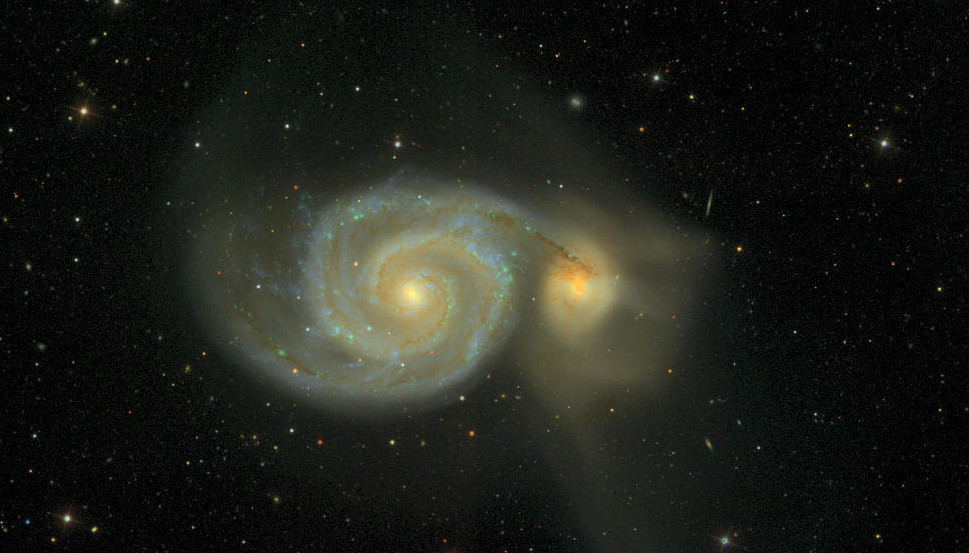
\includegraphics[width=0.8\textwidth]{M51-4x4-crop.jpg}
                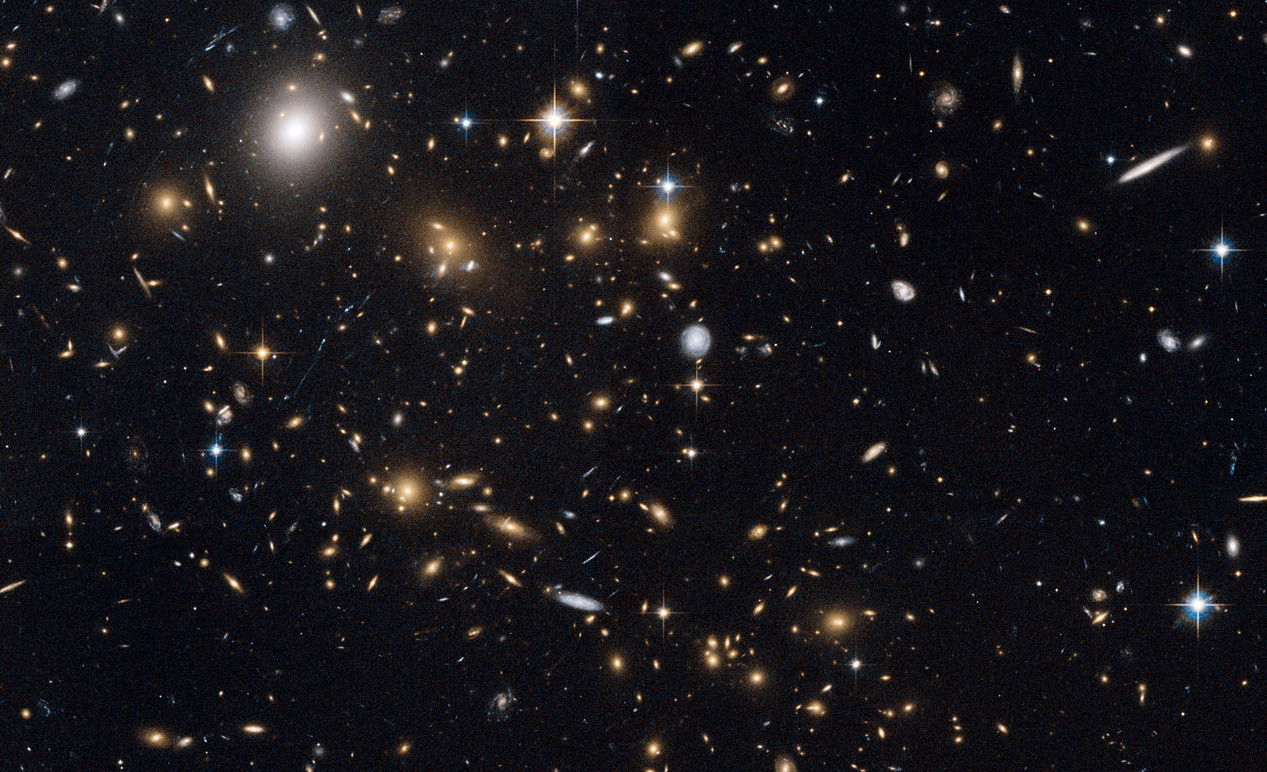
\includegraphics[width=0.8\textwidth]{macs-cluster-crop.jpg}
                \includegraphics[width=0.8\textwidth]{sdss-gals-blanton.jpg}
            \end{center}
        \end{column}
    \end{columns}
}

\frame
{
    \frametitle{Basic Cosmology Parameters}

    % \setbeamerfont*{itemize/enumerate body}{size=\Large}
    % \setbeamerfont*{itemize/enumerate subbody}{parent=itemize/enumerate body}
    % \setbeamerfont*{itemize/enumerate subsubbody}{parent=itemize/enumerate body}

    \begin{columns}
        \begin{column}{0.5\textwidth}    
            \begin{itemize}

                \item \grhom: the mass density of the universe $\sim 3 \times
                    10^{-3}$g/cm$^3$, or \gomegam$\sim 0.3$ in normalized
                    units (30\% of the total energy density)

                \item \gsigma: the variance of the mass field on 8 Mpc
                    scales, relative to the mean density $\sigma_8 \sim 0.8$

                \item \gH: the current expansion rate $\sim 70~ $km/s/Mpc:
                    things farther away are moving faster away\newline
                    {\color{cadetblue}(1 pc = 3.3 light years)}

                \item Age of the universe 13.8 billion years

            \end{itemize}
        \end{column}
        \begin{column}{0.5\textwidth}    
            \begin{center}
                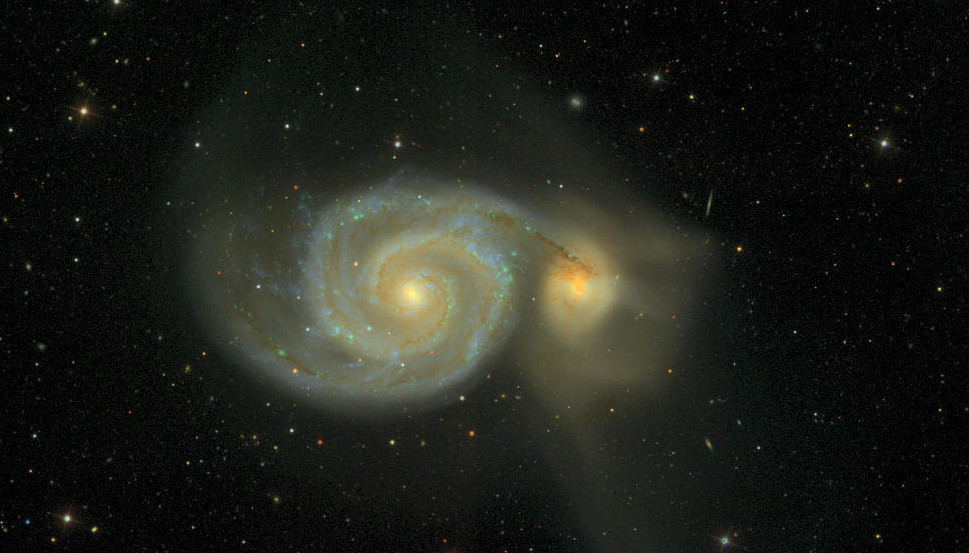
\includegraphics[width=0.8\textwidth]{M51-4x4-crop.jpg}
                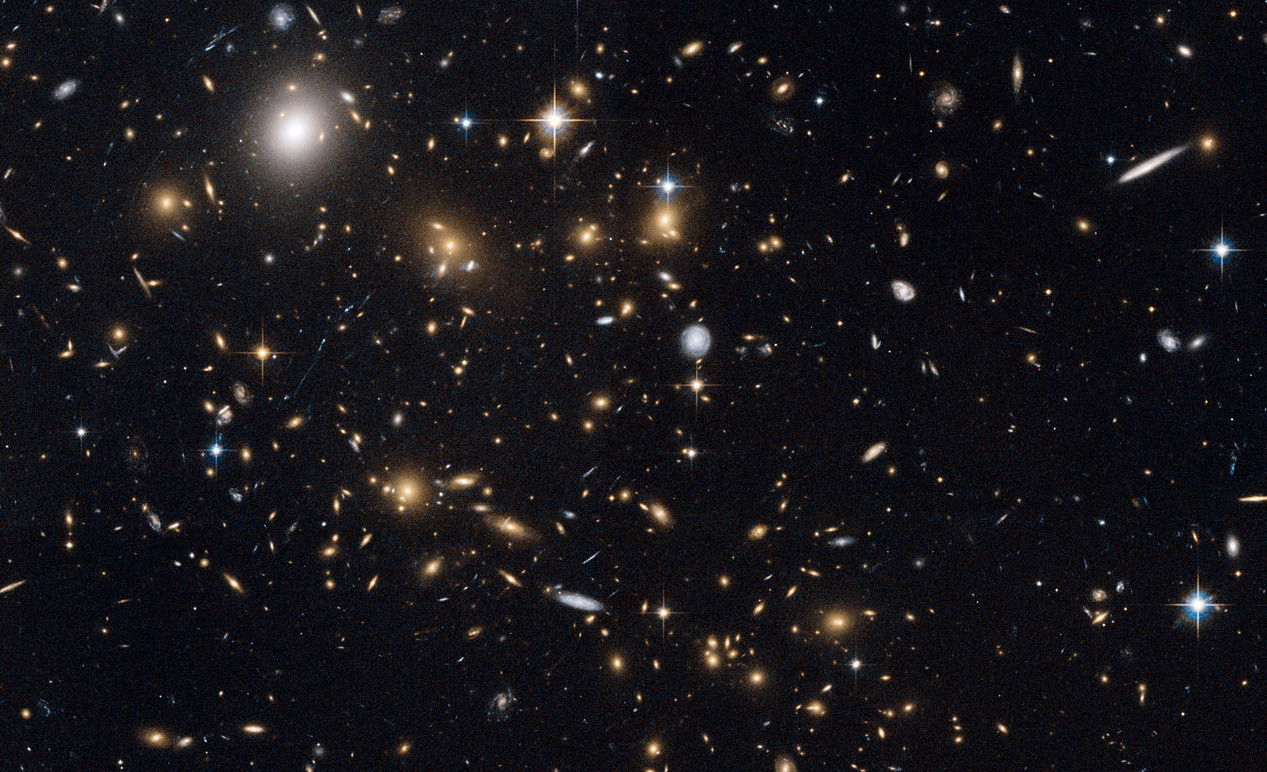
\includegraphics[width=0.8\textwidth]{macs-cluster-crop.jpg}
                \includegraphics[width=0.8\textwidth]{sdss-gals-blanton.jpg}
            \end{center}
        \end{column}
    \end{columns}
}

\frame
{
    \frametitle{Basic Cosmology Parameters}

    % \setbeamerfont*{itemize/enumerate body}{size=\Large}
    % \setbeamerfont*{itemize/enumerate subbody}{parent=itemize/enumerate body}
    % \setbeamerfont*{itemize/enumerate subsubbody}{parent=itemize/enumerate body}

    \begin{columns}
        \begin{column}{0.5\textwidth}    
            \begin{itemize}

                \item Convenient, well-constrained parameter combination {\color{gold} $S_8 = \sigma_8 \left( \Omega_m / 0.3 \right)^{0.5}$}

            \end{itemize}
        \end{column}
        \begin{column}{0.5\textwidth}    
            \begin{center}
                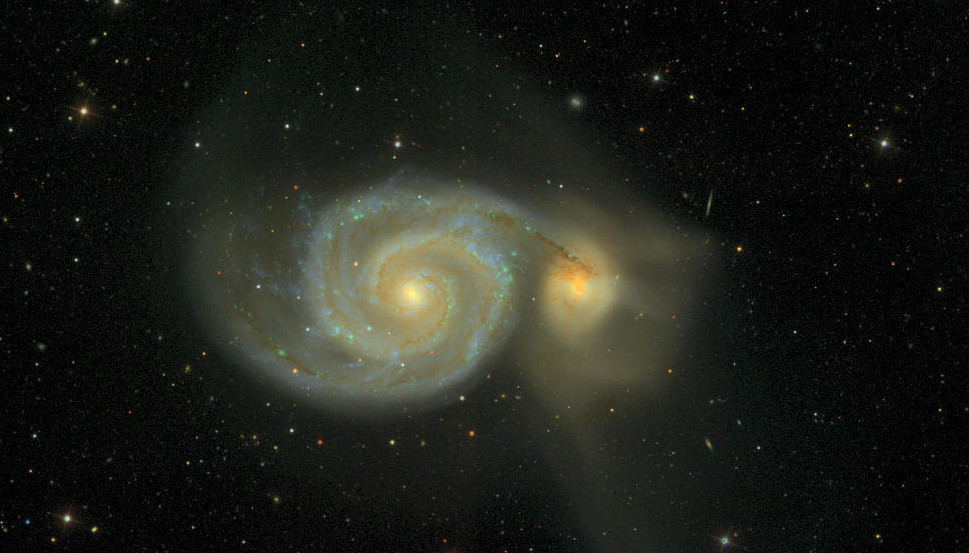
\includegraphics[width=0.8\textwidth]{M51-4x4-crop.jpg}
                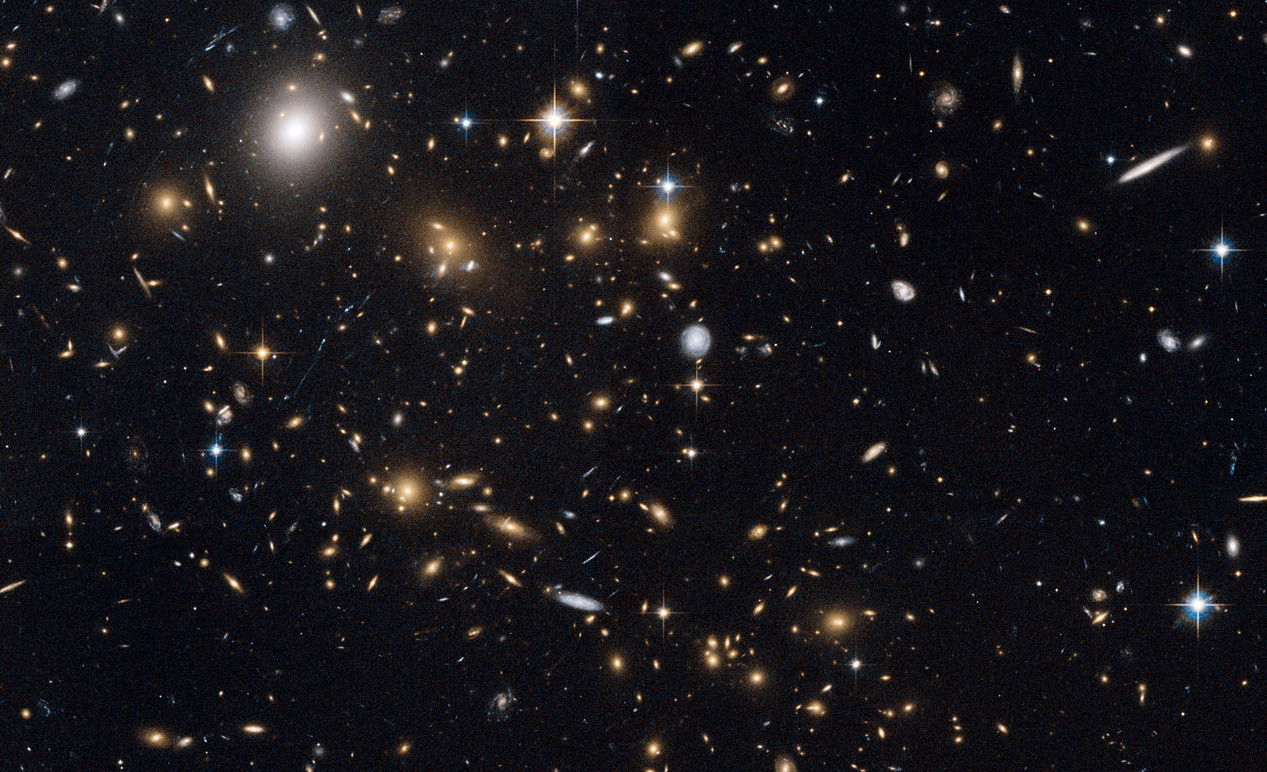
\includegraphics[width=0.8\textwidth]{macs-cluster-crop.jpg}
                \includegraphics[width=0.8\textwidth]{sdss-gals-blanton.jpg}
            \end{center}
        \end{column}
    \end{columns}
}


\frame
{
    \frametitle{Cosmology and Dark Energy}

    \setbeamerfont*{itemize/enumerate body}{size=\Large}
    \setbeamerfont*{itemize/enumerate subbody}{parent=itemize/enumerate body}
    \setbeamerfont*{itemize/enumerate subsubbody}{parent=itemize/enumerate body}

    \begin{itemize}

        \item Given initial conditions and the contents of the universe,
            we can explain much of what we see using General Relativity
            and Particle Physics

        \begin{itemize}
                
            \item Expansion history of the universe

            \item Light element abundance

            \item Relic background radiation from the big bang
                (Cosmic Microwave Background, CMB)

        \end{itemize}

    \item But there are a few mysteries.

    \end{itemize}
}

\frame
{
    \frametitle{Mysteries}

    \setbeamerfont*{itemize/enumerate body}{size=\Large}
    \setbeamerfont*{itemize/enumerate subbody}{parent=itemize/enumerate body}
    \setbeamerfont*{itemize/enumerate subsubbody}{parent=itemize/enumerate body}

    \begin{itemize}

        \item A few mysteries

        \begin{itemize}
                
            \item Why is the universe so homogeneous?  We know of no a priori 
                reason.  We invented {\color{gold} Inflation}.

            \item For a consistent picture we need a lot more matter than we {\it see},
                or a new theory of gravity.  We invented {\color{gold} Dark Matter}.

            \item The expansion of the universe appears to be accelerating
                rather than decelerating.  We invented {\color{gold} Dark Energy}.

        \end{itemize}

    \end{itemize}
}

{
    \definecolor{mblack}{RGB}{0,0,0}
    \setbeamertemplate{background canvas}[vertical shading][bottom=black,top=black]


    \frame
    {
        The universe {\em is} homogeneous
        \begin{columns}[T]
            \begin{column}{0.55\textwidth}
                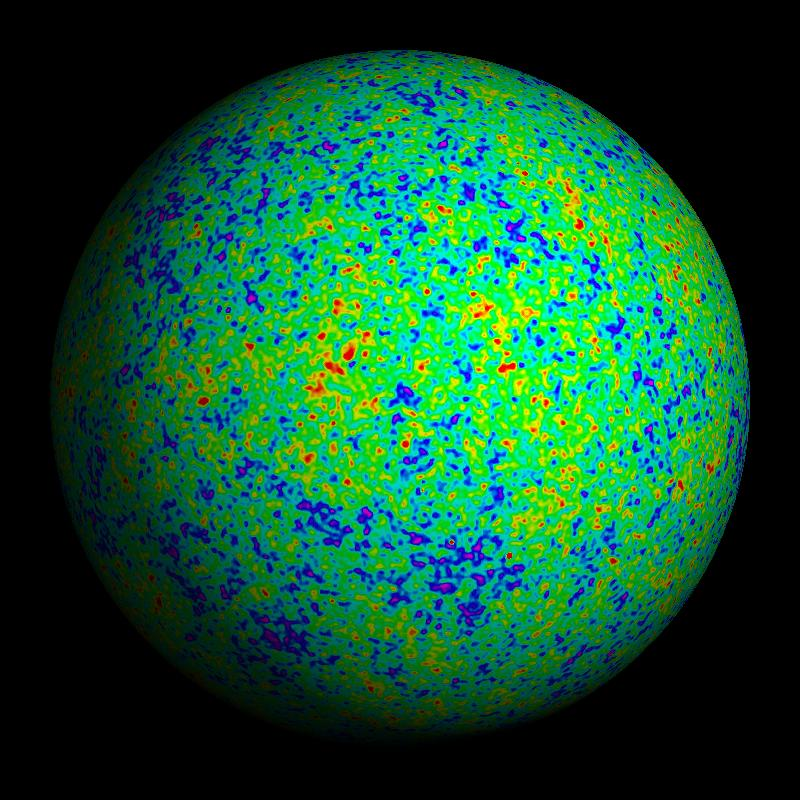
\includegraphics[trim=50 50 50 50,clip,width=\textwidth]{CMB-Tegmark.jpeg}
            \end{column}
            \begin{column}{0.55\textwidth}
                \vspace{10 mm}
                \includegraphics[width=\textwidth]{sdss-gals-blanton.jpg}
            \end{column}
        \end{columns}
        {\tiny \hfill WMAP (M. Tegmark), SDSS Galaxies (M. Blanton)}
    }
    \definecolor{mblack}{RGB}{50,50,50}
    \setbeamertemplate{background canvas}[vertical shading][bottom=mgray,top=mblack]

}




\frame
{
    \frametitle{The Accelerating Universe}

    \begin{columns}
        \begin{column}{0.5\textwidth}    
            \begin{itemize}

                \item Discovered using a type of supernova that is a ``standard
                    candle'', given their apparent brightness we can determine
                    how far away they are (Riess et al. 1998, Perlmutter et al. 1999)
                        
                \item The curve of brightness vs. distance doesn't look right.

                \item Implies that the universe decelerated early on,
                    but began to accelerate later.

            \end{itemize}
        \end{column}
        \begin{column}{0.5\textwidth}    
            \begin{center}
                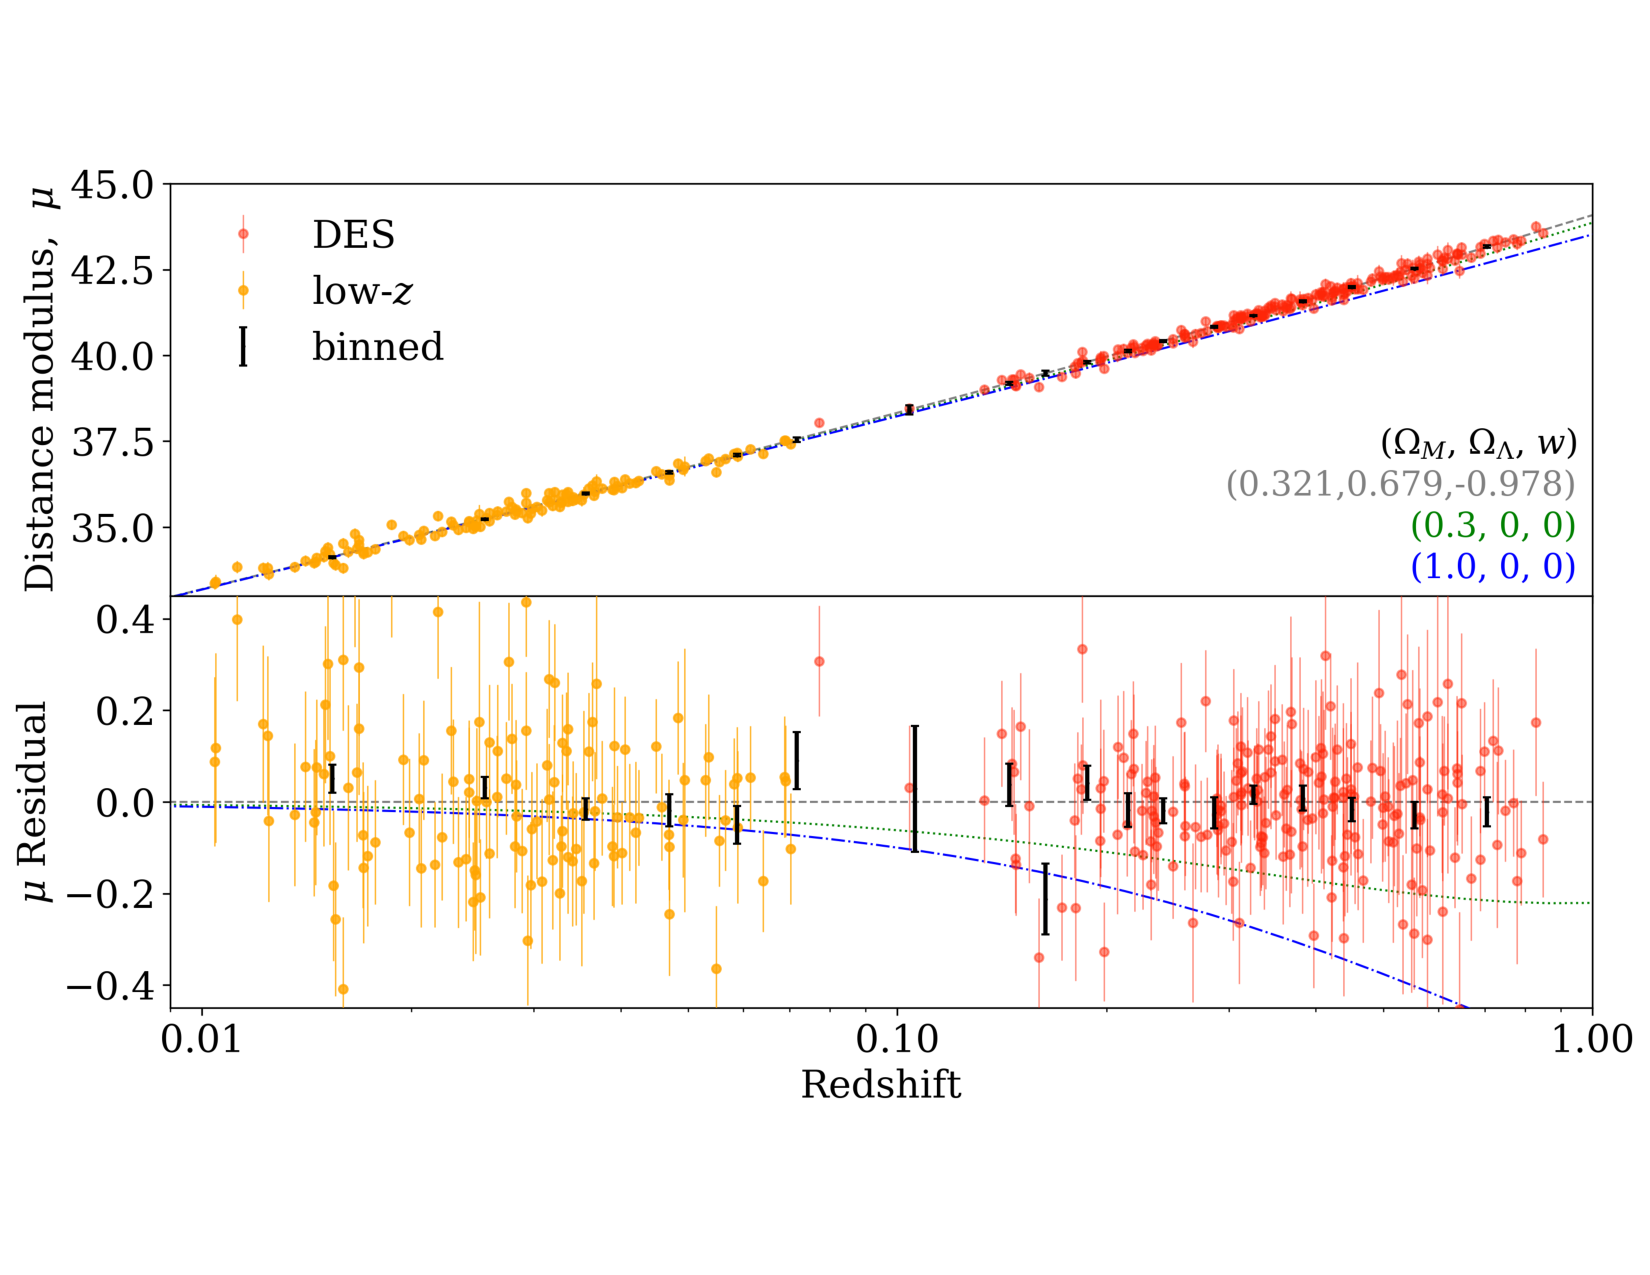
\includegraphics[width=\textwidth]{hubble_diagram_combined.pdf}
                {\tiny Dark Energy Survey, Abbott et al. 2018}
            \end{center}
        \end{column}
    \end{columns}

}

\frame
{
    \frametitle{Why is this a mystery?}

    \begin{itemize}
        \item We can use the Einstein field equations to derive the
            acceleration.
            % \begin{equation}
            %     G_{\mu, \nu} = \frac{8 \pi G}{c^4} T_{\mu, \nu}
            % \end{equation}
            \begin{equation}
                G_{\mu, \nu} \propto T_{\mu, \nu}
            \end{equation}
            Putting in a homogeneous and isotropic universe with
            density $\rho_m(t)$ we can
            derive the dynamics for, say, the distance $R$ between
            two distant galaxies
            % \begin{equation}
            %     \ddot{R} = -\frac{4 \pi G c^2}{3} R(t) \rho(t)
            % \end{equation}
            \begin{equation}
                \ddot{R} \propto - R(t) \rho_m(t)
            \end{equation}

        \item All the terms on the right hand side are positive!
    \end{itemize}
}

\frame
{
    \frametitle{What did we leave out?}

    \begin{itemize}
        \item We could include pressure {\color{gold} $p(t)$} as well
            % \begin{equation}
            %     \ddot{R} = -\frac{4 \pi G c^2}{3} R(t) \left[\rho(t) + \frac{3}{c^2} {\color{gold} p(t)}\right]
            % \end{equation}
            \begin{equation}
                \ddot{R} \propto - R(t) \left[\rho_m(t) + 3~ {\color{gold} p_m(t)}\right]
            \end{equation}
            But normal matter (stars, diffuse gas) has $p_m \sim 0$
            and even if it did have pressure it has the wrong sign.  The equation
            of state for normal matter is
            \begin{align}
                p_m &= w_m \times \rho_m \\
                w_m & > 0
            \end{align}
            Note: I've set $c = 1$

        \item So the pressure would not come from matter but some new substance or field, 
            people call it \gdarkenergy, with $p = w \times \rho$

        \item We need $w < -1/3$ to get any acceleration

    \end{itemize}
}

\frame
{
    \frametitle{What did we leave out?}

    \begin{itemize}
        \item We could include Einstein's cosmological constant fudge factor
            \glambda\ (ironically introduced to keep the universe static)
            % \begin{equation} 
            %     G_{\mu, \nu} + \Lambda g_{\mu, \nu} = \frac{8 \pi G}{c^4} T_{\mu, \nu}
            % \end{equation}
            \begin{equation} 
                G_{\mu, \nu} + \glambda\ g_{\mu, \nu} \propto T_{\mu, \nu}
            \end{equation}

            % \begin{equation}
            %     \ddot{R} = -\frac{4 \pi G c^2}{3} R(t) \left[\rho(t) + \frac{3}{c^2} {\color{gold} p(t)} - \frac{{\color{gold} \Lambda}}{3}\right]
            % \end{equation}
            % \begin{equation}
            %     \ddot{R} \propto R(t) \left[\rho(t) + 3 ~ {\color{gold} p(t)} - \frac{{\color{gold} \Lambda}}{3}\right]
            % \end{equation}
            \begin{equation}
                \ddot{R} \propto R(t) \left[\rho_m + {\color{gold} \rho(t) + 3 ~ p(t)} - \frac{\glambda}{4 \pi G}\right]
            \end{equation}
            %(just showing Dark Energy and \glambda).

        \item Either we need a positive cosmological constant {\color{gold} $\Lambda$}
            or we need some bizarre field \gdarkenergy\ with negative pressure {\color{gold}
            $p(t) = w \times \rho(t), ~ w < -1/3$}.

        \item If this component is small compared to the matter density \grhom\
            in the early universe, but comes to dominate later, we can explain
            the universe decelerating then accelerating.

    \end{itemize}
}

\frame
{
    \frametitle{Is it {\color{gold} $\Lambda$} or Dark Energy?}

    \setbeamerfont*{itemize/enumerate body}{size=\Large}
    \setbeamerfont*{itemize/enumerate subbody}{parent=itemize/enumerate body}
    \setbeamerfont*{itemize/enumerate subsubbody}{parent=itemize/enumerate body}

    \begin{itemize}

        \item $p = w \times \rho$

        \item \glambda\ is equivalent to a constant ${\color{gold}w = -1}$,
            and is spatially homogeneous and isotropic.

        \item Dark Energy could have any ${\color{gold} w(t) < -1/3}$ to
            produce acceleration.  Not required to be perfectly homogeneous
            and isotropic.

    \end{itemize}
}


\frame
{
    \frametitle{What do we know at this point?}

    \setbeamerfont*{itemize/enumerate body}{size=\Large}
    \setbeamerfont*{itemize/enumerate subbody}{parent=itemize/enumerate body}
    \setbeamerfont*{itemize/enumerate subsubbody}{parent=itemize/enumerate body}

    \begin{columns}
        \begin{column}{0.5\textwidth}    
            \begin{itemize}

                \item Great progress in the last 20 years!

                \item We don't currently have enough information to tell if
                    it is \glambda\ or \gdarkenergy.

                \item We need more data.  In cosmology this means {\it surveys}.

            \end{itemize}
        \end{column}
        \begin{column}{0.5\textwidth}    
            %\begin{center}
                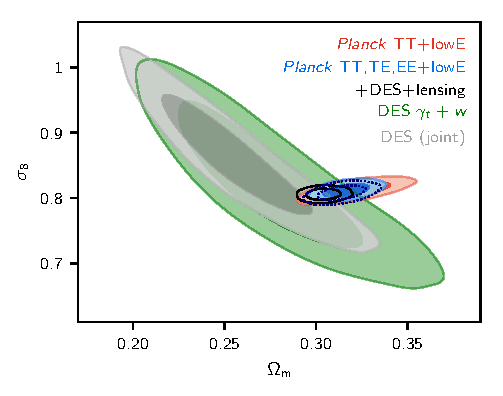
\includegraphics[width=0.9\textwidth]{DES-joint-s8-omm.pdf}
                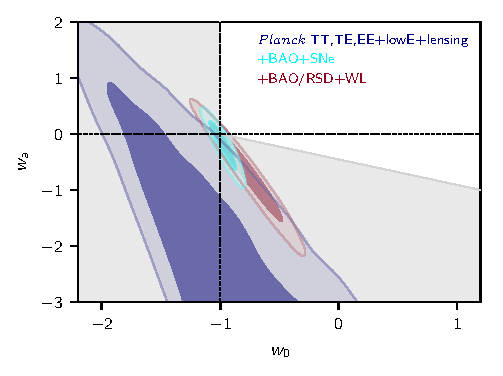
\includegraphics[width=0.9\textwidth]{w0_wa.pdf}
                \newline
                {\tiny Planck Collaboration 2018}
            %\end{center}

        \end{column}
    \end{columns}
}

\frame
{

    \frametitle{Dark Energy Survey (DES)}

    \fontsize{9}{0.8\baselineskip}

    \begin{columns}

        \begin{column}{0.4\textwidth}
            \includegraphics[scale=0.17]{ctio_blanco_crew_2013Oct-30-small-balance.jpg}
            \newline
            \hfill {\tiny Image: Brian Nord, FNAL}
        \end{column}


        \begin{column}{0.6\textwidth}

            \begin{itemize}

                \item Imaging survey of 5000 square degrees in the southern
                    sky in Chile.  5 optical filters

                \item New 500 Megapixel camera

                \item First light Fall 2012, data taking now finished

                \item Study Dark Energy using weak gravitational lensing,
                    clustering of galaxies and supernovae.

            \end{itemize}

        \end{column}

    \end{columns}

}

{
	\definecolor{mblack}{RGB}{0,0,0}
    \setbeamertemplate{background canvas}[vertical shading][bottom=black,top=black]
	
    \frame
    {

        \begin{center}
            \includegraphics[width=1.1\textwidth]{DES-2013-01-medres.jpg}

            {\tiny \hfill NGC 1398, Erin Sheldon, Martin Murphy, DES}
        \end{center}
    }

	\definecolor{mblack}{RGB}{50,50,50}
    \setbeamertemplate{background canvas}[vertical shading][bottom=mgray,top=mblack]

}

{
	\definecolor{mblack}{RGB}{0,0,0}
    \setbeamertemplate{background canvas}[vertical shading][bottom=black,top=black]
	
    \frame
    {

        \begin{center}
            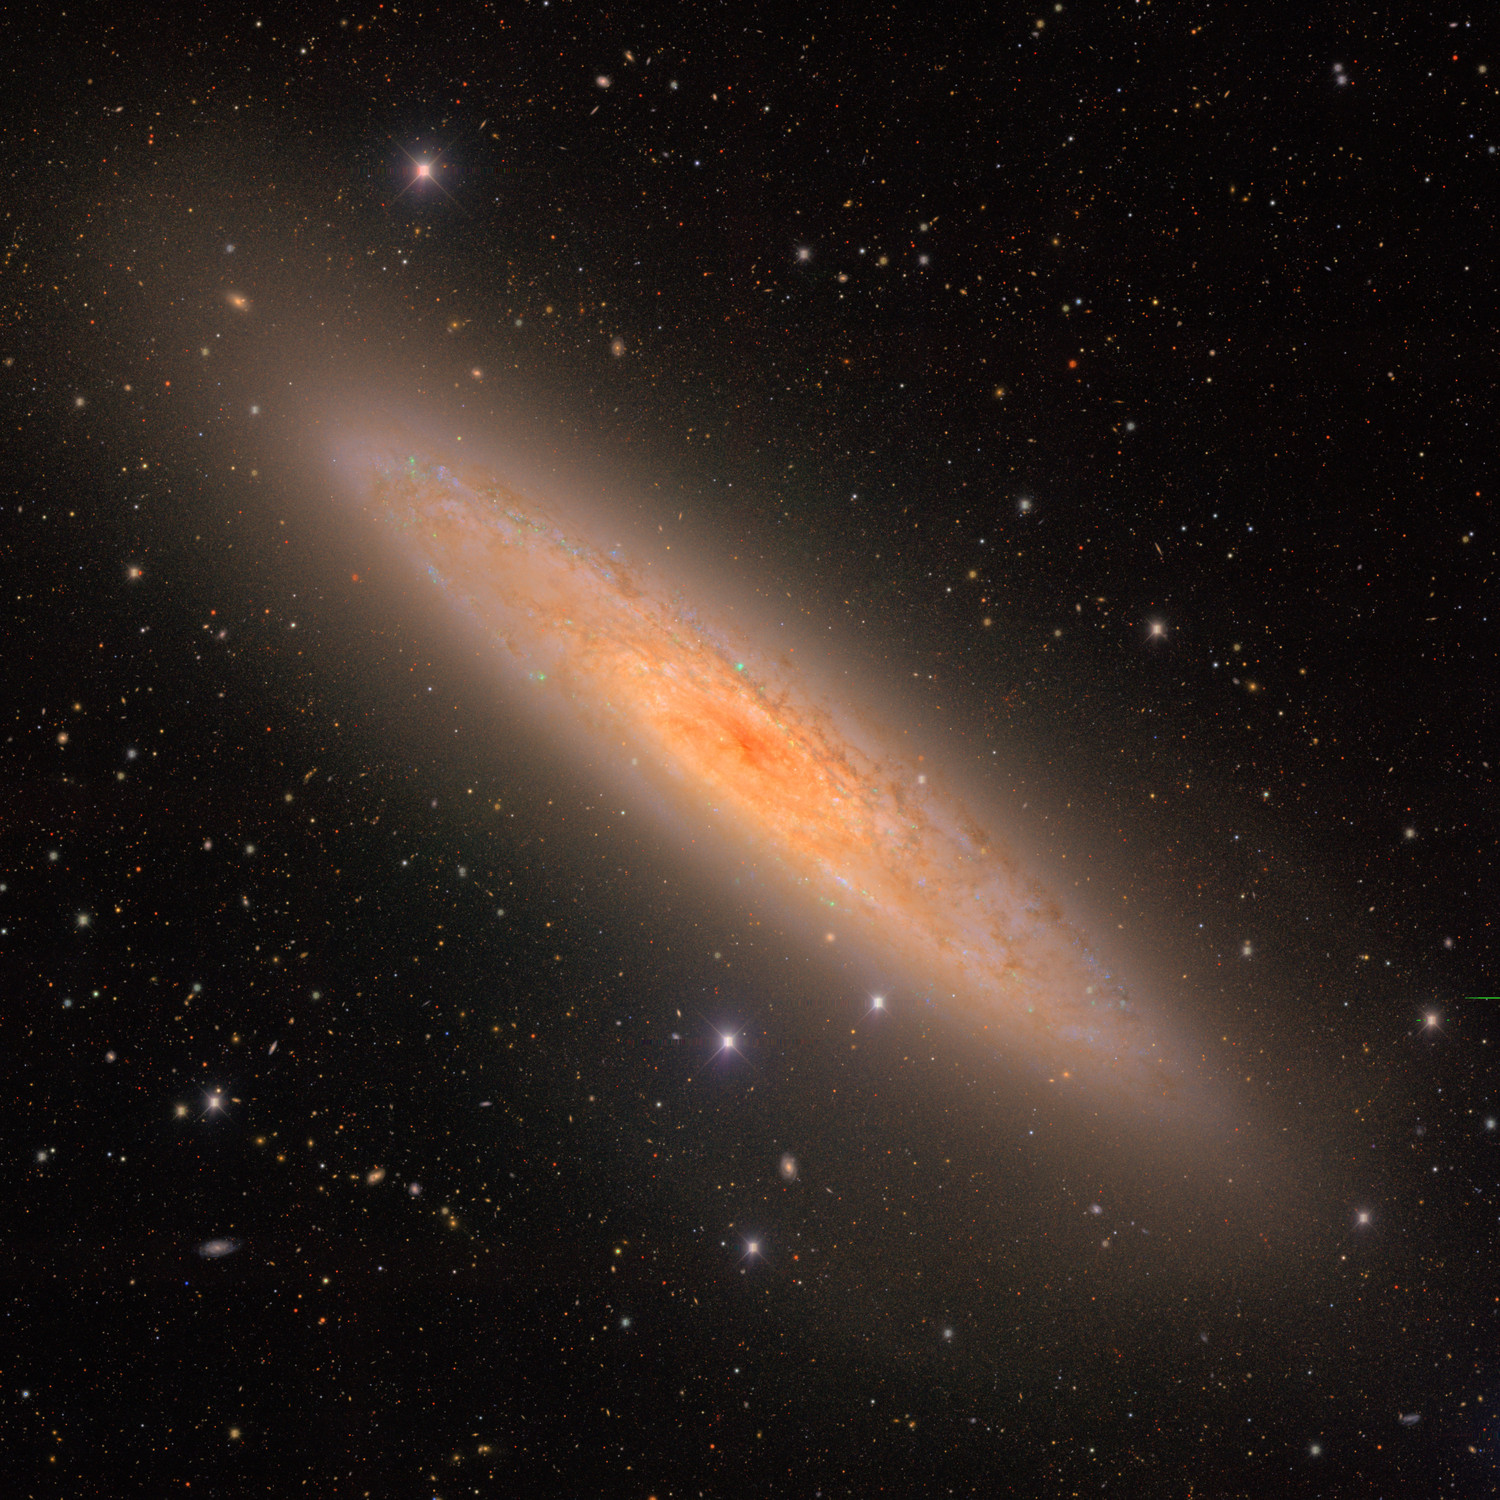
\includegraphics[width=0.81\textwidth]{ngc0253-small.jpg}

            {\tiny \hfill NGC 0253, Erin Sheldon, DES}
        \end{center}
    }

	\definecolor{mblack}{RGB}{50,50,50}
    \setbeamertemplate{background canvas}[vertical shading][bottom=mgray,top=mblack]

}

{
	\definecolor{mblack}{RGB}{0,0,0}
    \setbeamertemplate{background canvas}[vertical shading][bottom=black,top=black]
	
    \frame
    {

        \begin{center}
            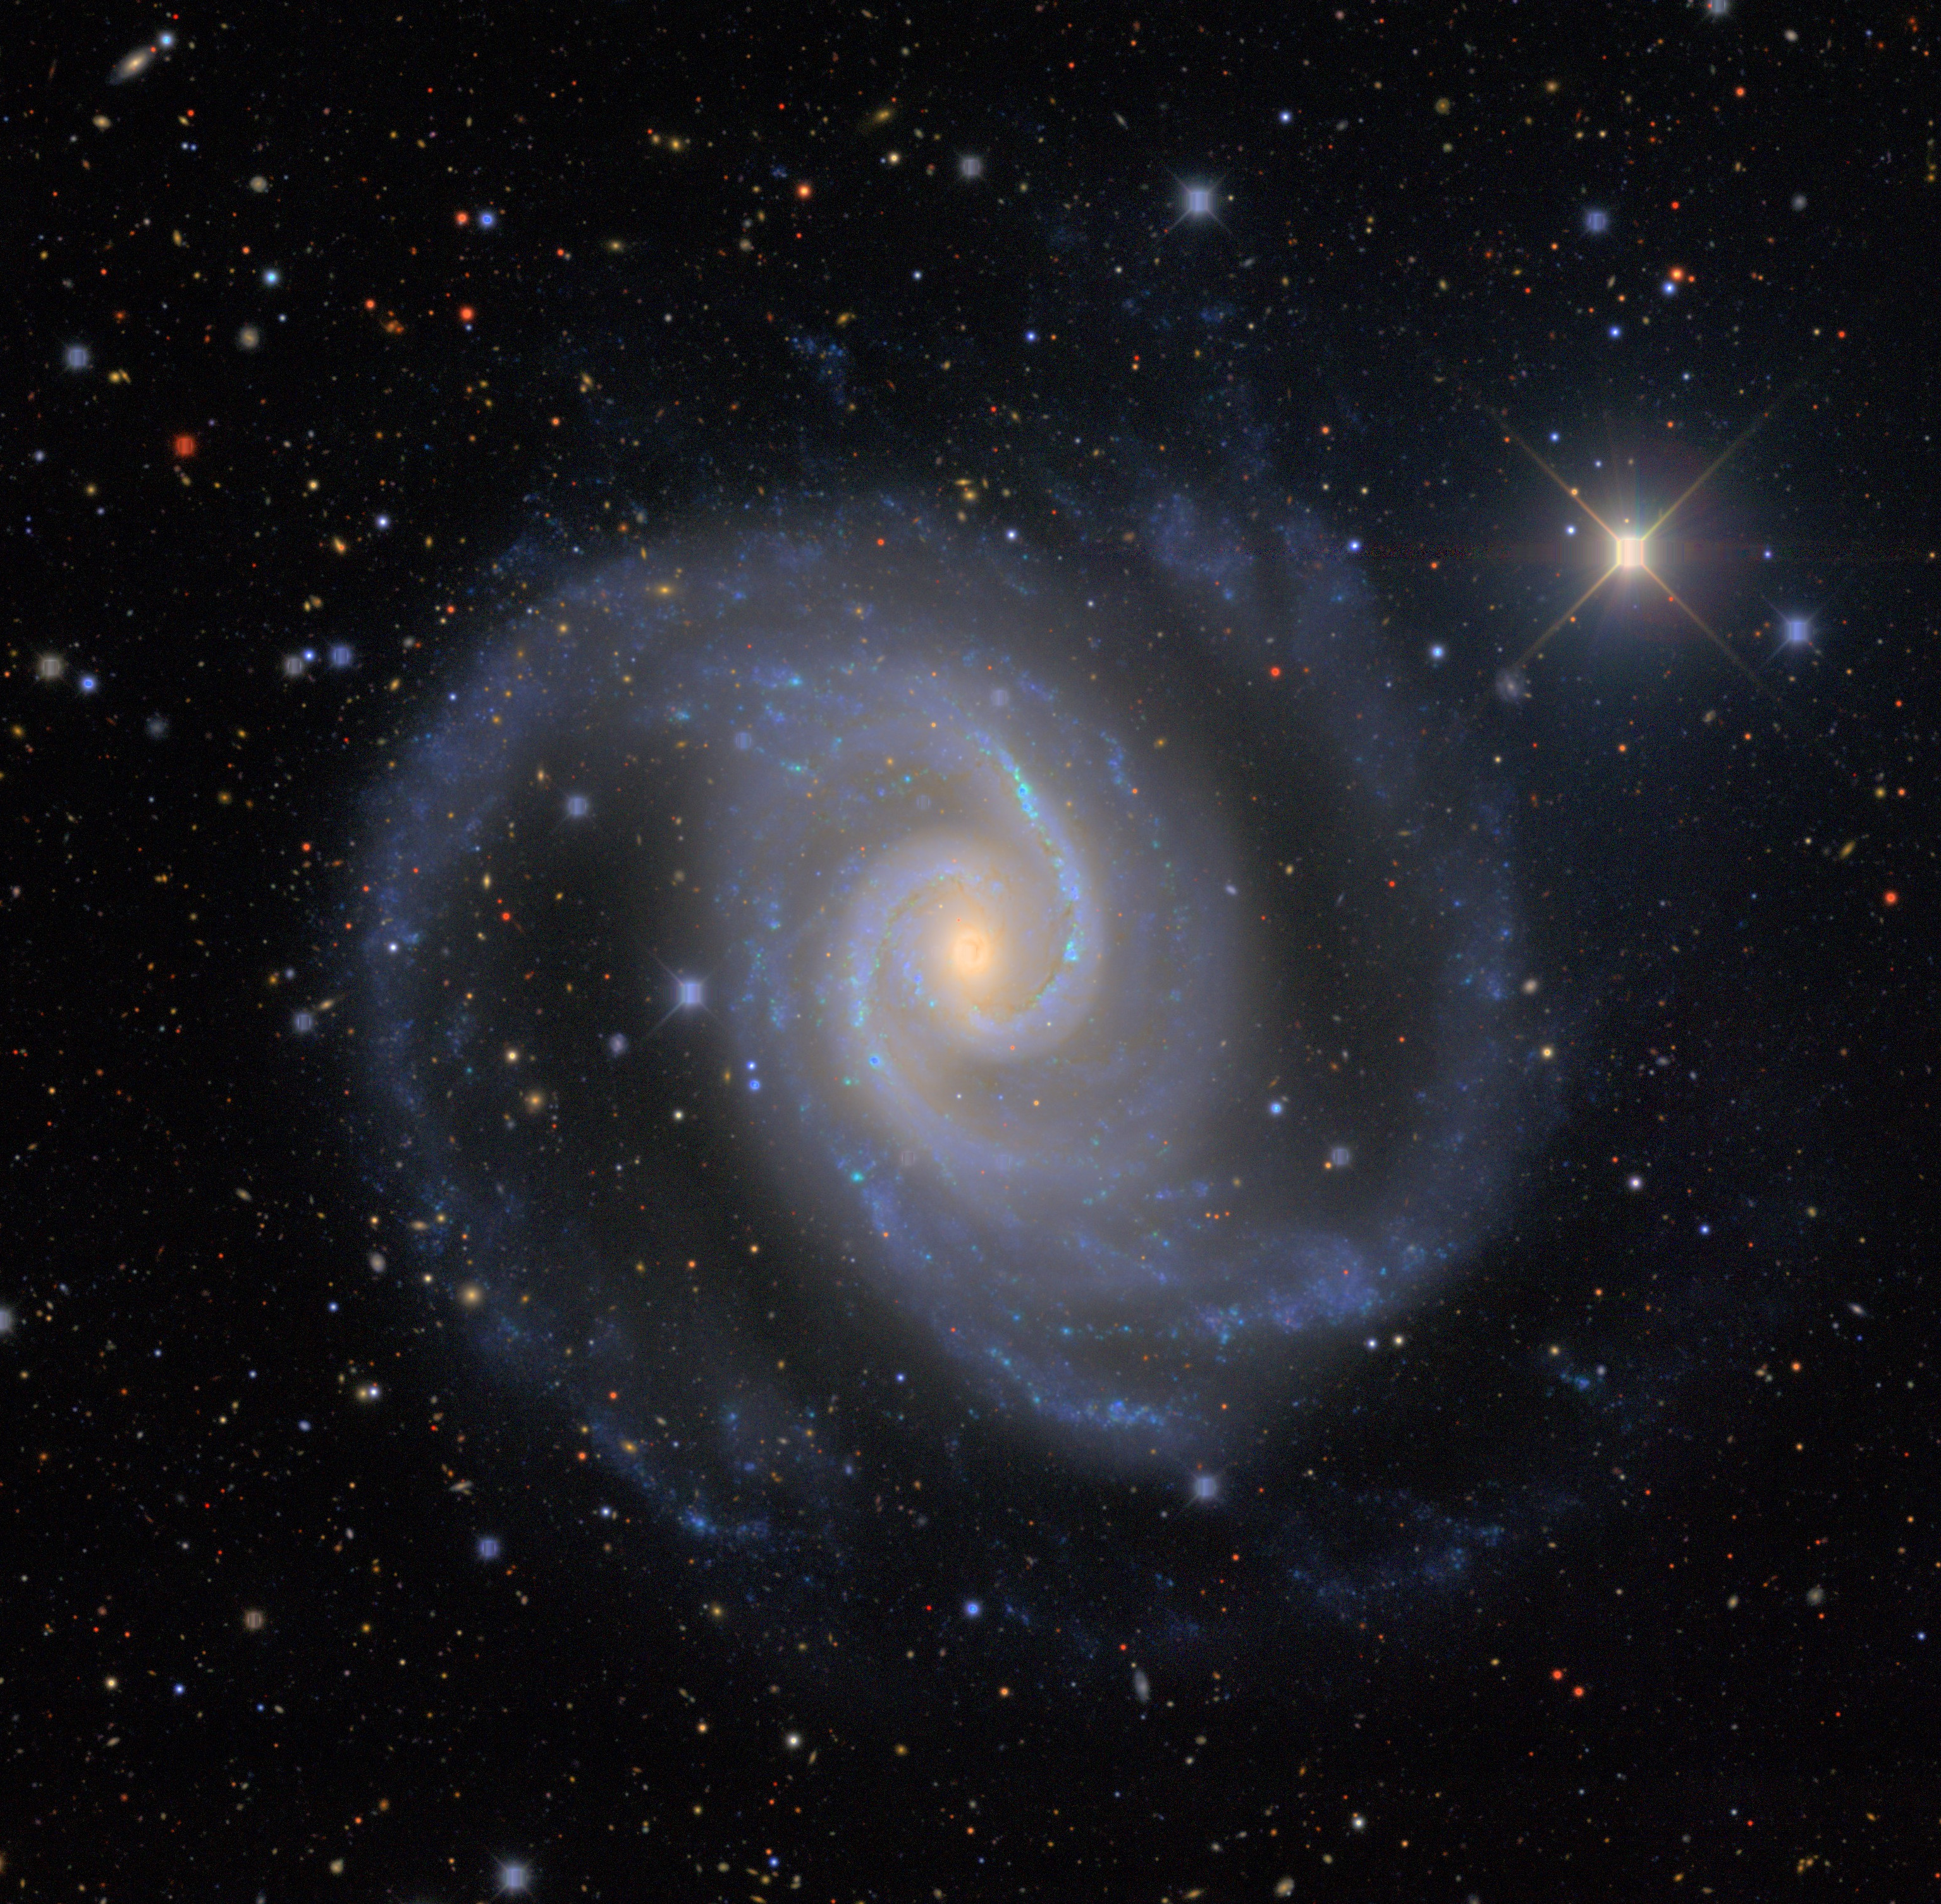
\includegraphics[width=0.81\textwidth]{DES0421-5457-gri-ngc1566.jpg}

            {\tiny \hfill NGC 1566, Erin Sheldon, DES}
        \end{center}
    }

	\definecolor{mblack}{RGB}{50,50,50}
    \setbeamertemplate{background canvas}[vertical shading][bottom=mgray,top=mblack]

}

{
	\definecolor{mblack}{RGB}{0,0,0}
    \setbeamertemplate{background canvas}[vertical shading][bottom=black,top=black]
	
    \frame
    {

        \begin{center}
            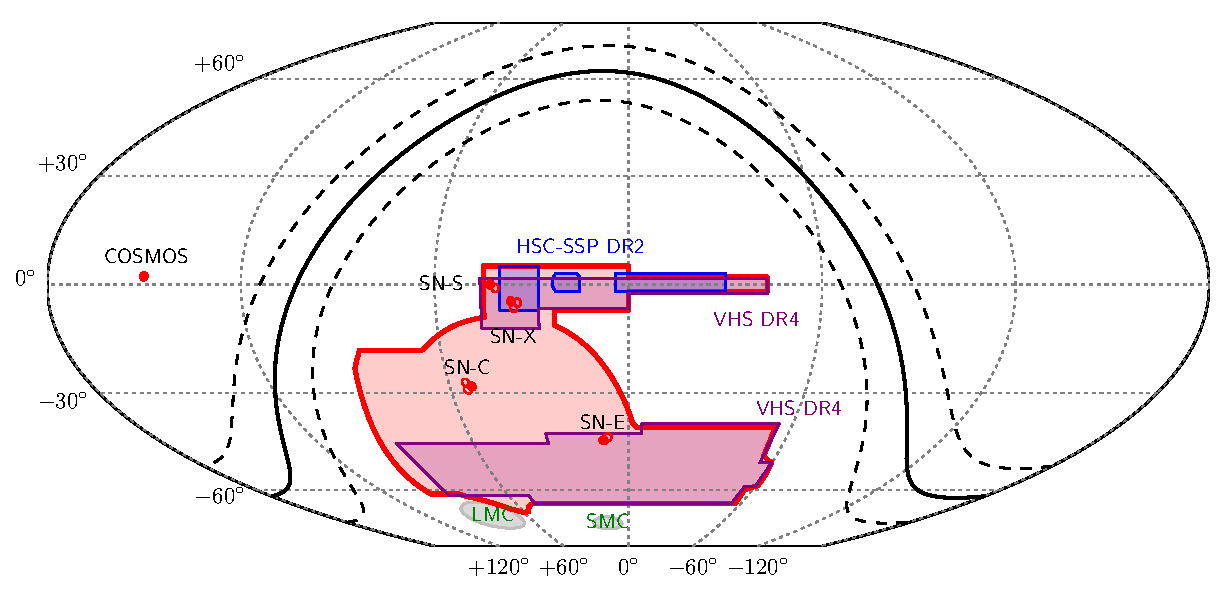
\includegraphics[width=1.0\textwidth]{des_footprint_v6.pdf}

            {\tiny \hfill I. Sevilla-Noarbe, DES}
        \end{center}
    }

	\definecolor{mblack}{RGB}{50,50,50}
    \setbeamertemplate{background canvas}[vertical shading][bottom=mgray,top=mblack]

}

{
	\definecolor{mblack}{RGB}{0,0,0}
    \setbeamertemplate{background canvas}[vertical shading][bottom=black,top=black]

    \frame
    {

        \begin{center}
            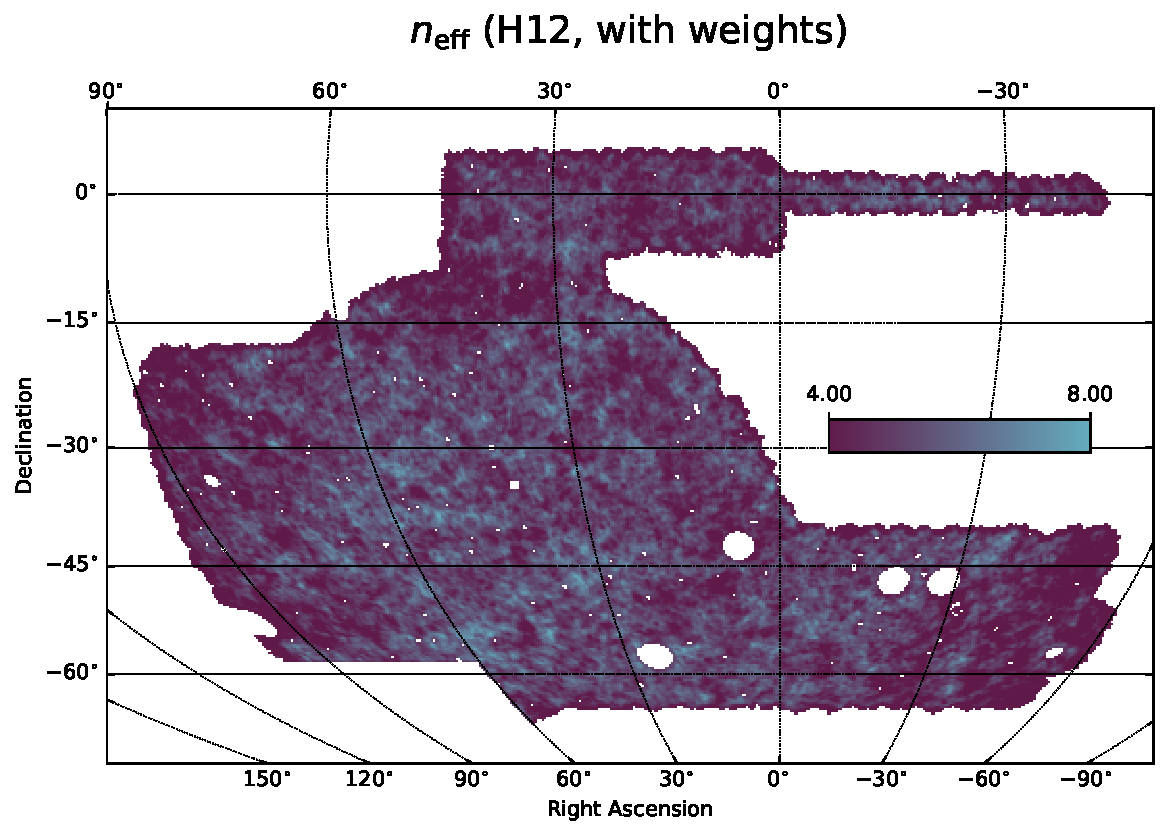
\includegraphics[width=0.6\textwidth]{neffw.pdf}

            {\tiny \hfill M. Gatti, DES}
        \end{center}
        \begin{itemize}

            \item 400 million objects

            \item State-of-the-art calibration of object flux and positions

        \end{itemize}
    }

	\definecolor{mblack}{RGB}{50,50,50}
    \setbeamertemplate{background canvas}[vertical shading][bottom=mgray,top=mblack]

}

{
	\definecolor{mblack}{RGB}{0,0,0}
    \setbeamertemplate{background canvas}[vertical shading][bottom=black,top=black]
	
    \frame
    {

        \begin{center}
            \includegraphics[width=1.1\textwidth]{members.png}

            {\tiny \hfill DES Members}
        \end{center}
    }

	\definecolor{mblack}{RGB}{50,50,50}
    \setbeamertemplate{background canvas}[vertical shading][bottom=mgray,top=mblack]

}


\frame
{

    {\Huge Gravitational Lensing}

}


\frame
{

    {\Large 
        {\em Do not Bodies act upon light at a distance, and by their action bend its Rays;
        and is not this action } (caeteris paribus) {\em strongest at the least distance?}
        \newline

        \hfill - Isaac Newton (Query I, Opticks, 1704)
    }
}

\frame
{
    \frametitle{Gravitational Lensing}

    \setbeamerfont*{itemize/enumerate body}{size=\large}
    \setbeamerfont*{itemize/enumerate subbody}{parent=itemize/enumerate body}
    \setbeamerfont*{itemize/enumerate subsubbody}{parent=itemize/enumerate body}
 
    \begin{itemize}

        \item Newton's first Query, Opticks, 1704
            \begin{itemize}
                \item One can naively ``cancel'' the zero masses and predict
                    bending of light rays, but mathematically bogus
            \end{itemize}

        \item Einstein 1911
            \begin{itemize}

                \item Equivalence principle

                \item Observers in free fall experience an inertial frame.  The
                    light appears to follow straight lines: the light falls
                    with them.

            \end{itemize}

        \item Einstein 1915
            \begin{itemize}
                \item Full result from general relativity, factor of two larger
            \end{itemize}


    \end{itemize}

}


%{
%	\definecolor{mblack}{RGB}{0,0,0}
%    \setbeamertemplate{background canvas}[vertical shading][bottom=black,top=black]
	
    \frame
    {
        \frametitle{1919 Eclipse}

        %\fontsize{9}{0.8\baselineskip}
        \begin{columns}
            \begin{column}{0.5\textwidth}    
                \begin{itemize}

                    \item Einstein predicted the light from background stars would
                        be deflected as it passes near the sun.

                    \item Eddington and colleagues observed the 1919 eclipse
                        looking for the effect.

                    \item The locations of stars with known positions were
                        measured, and found to have moved

                \end{itemize}
            \end{column}
            \begin{column}{0.5\textwidth}
                \begin{center}
                    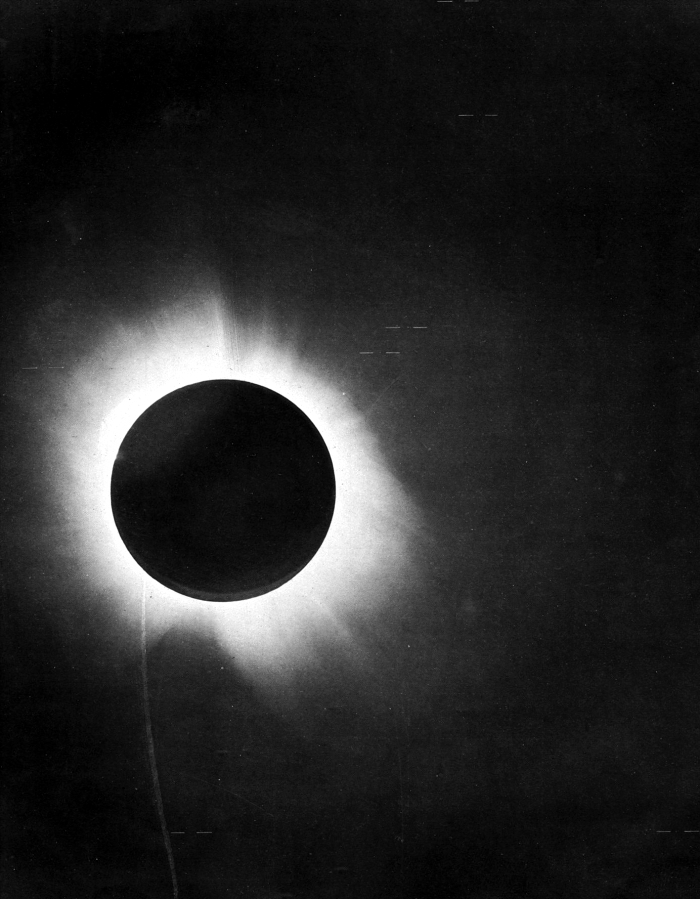
\includegraphics[width=\textwidth]{1919_eclipse_positive.jpg}
                    \newline
                    {\tiny Dyson, Eddington, Davidson 1919}
                \end{center}
            \end{column}
        \end{columns}
    }

%	\definecolor{mblack}{RGB}{50,50,50}
%    \setbeamertemplate{background canvas}[vertical shading][bottom=mgray,top=mblack]

%}

\frame
{
    \frametitle{Lensing Geometry}

    \begin{center}
        
\includegraphics[scale=0.4]{lens_geometry_invert.pdf}
        \newline
        For a point mass lens, the deflection depends on impact
        prameter and mass as
        \newline
        {\huge {\color{gold} $\alpha \propto \frac{M}{b}$ }}
    \end{center}
}



\frame
{
    \frametitle{Twin Quasar 0957+0561}

    %\fontsize{9}{0.8\baselineskip}
    \begin{columns}
        \begin{column}{0.5\textwidth}    
            \begin{itemize}

                \item Two interesting quasars discovered in 1979 (Walsh, Carswell, Weyman)

                \item Extremely close together, nearly identical spectrum and redshift

                \item Time variations in image A appear in image B also, but 14 months later.

                \item Two images of the same object!
                    
            \end{itemize}
        \end{column}
        \begin{column}{0.5\textwidth}
            \begin{center}
                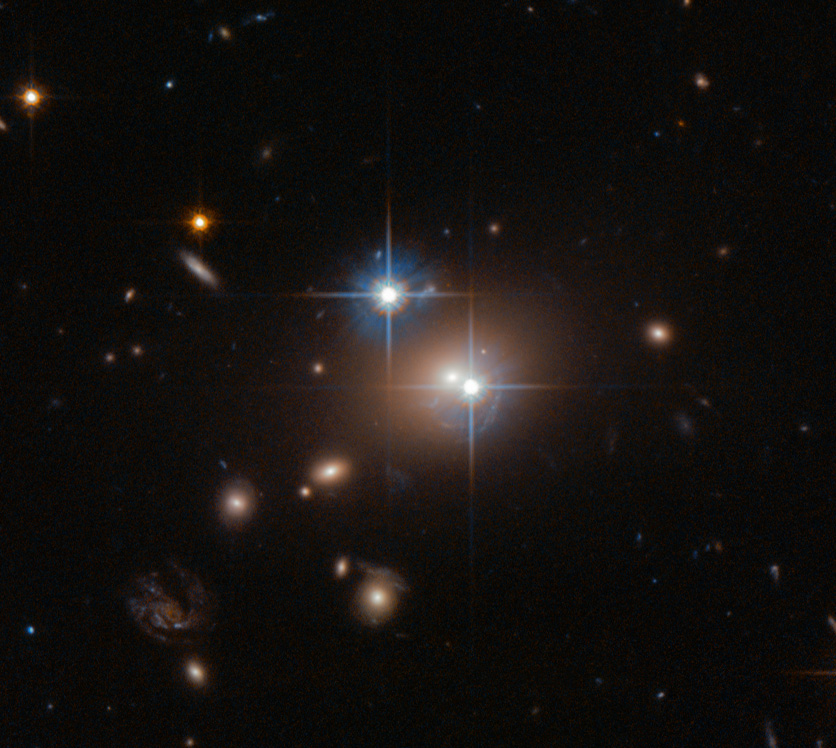
\includegraphics[width=\textwidth]{QSO_B0957+0561-crop.jpg}
                \newline
                {\tiny ESA/Hubble \& NASA}
            \end{center}
        \end{column}
    \end{columns}
}

\frame
{
    \frametitle{Twin Quasars: {\color{gold} Can infer $\alpha$}}

    \begin{center}
        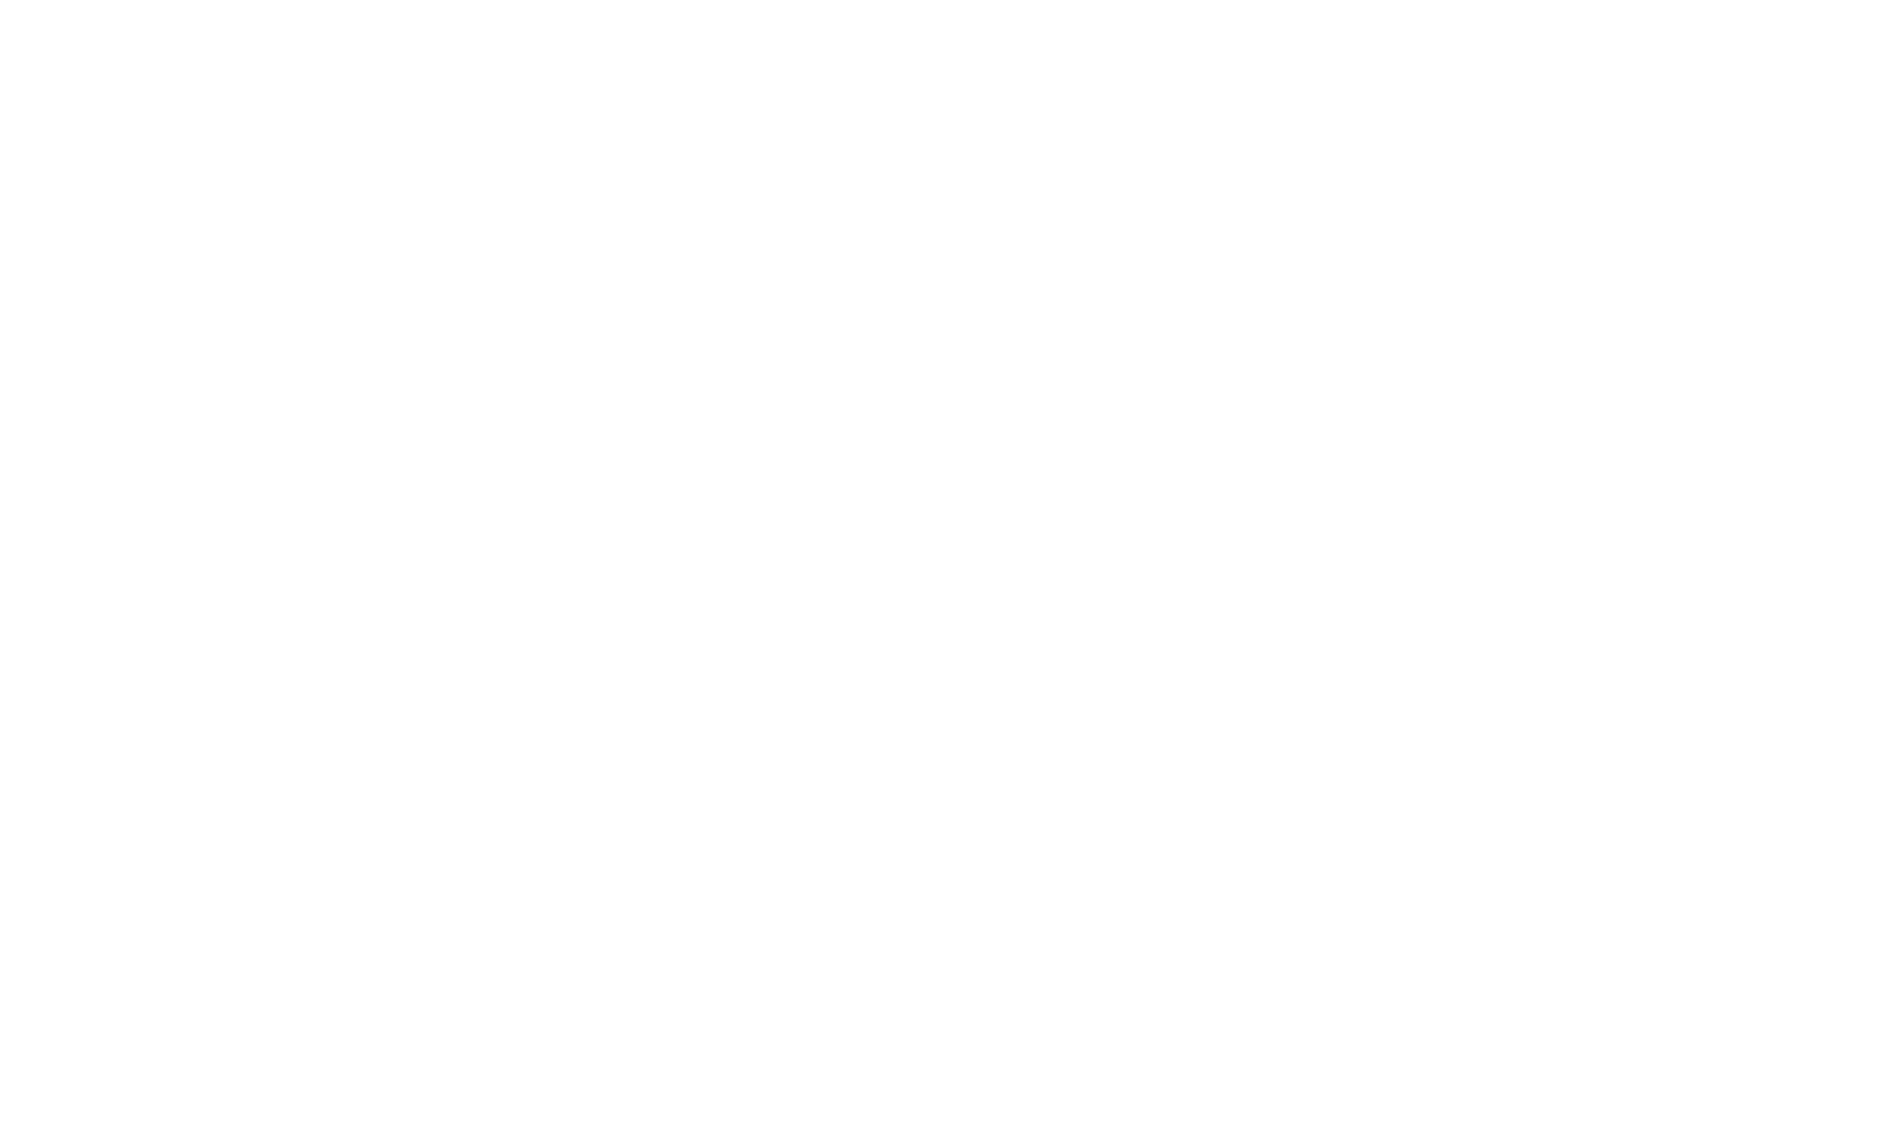
\includegraphics[width=\textwidth]{glensing.png}
    \end{center}
        %\newline
        \hfill  {\tiny User Krishnavedala, {\em wikipedia} }
}


{
	\definecolor{mblack}{RGB}{0,0,0}
    \setbeamertemplate{background canvas}[vertical shading][bottom=black,top=black]
	
    \frame
    {
        \frametitle{Einstein Ring: The ``Horseshoe''}

        \begin{center}
            \includegraphics[height=0.7\textheight]{A_Horseshoe_Einstein_Ring_from_Hubble.JPG}

            {\tiny \hfill ESA/Hubble \& NASA}
        \end{center}
    }

	\definecolor{mblack}{RGB}{50,50,50}
    \setbeamertemplate{background canvas}[vertical shading][bottom=mgray,top=mblack]

}


{
	\definecolor{mblack}{RGB}{0,0,0}
    \setbeamertemplate{background canvas}[vertical shading][bottom=black,top=black]
	
    \frame
    {
        \frametitle{Shear Illustration}
        \begin{center}
            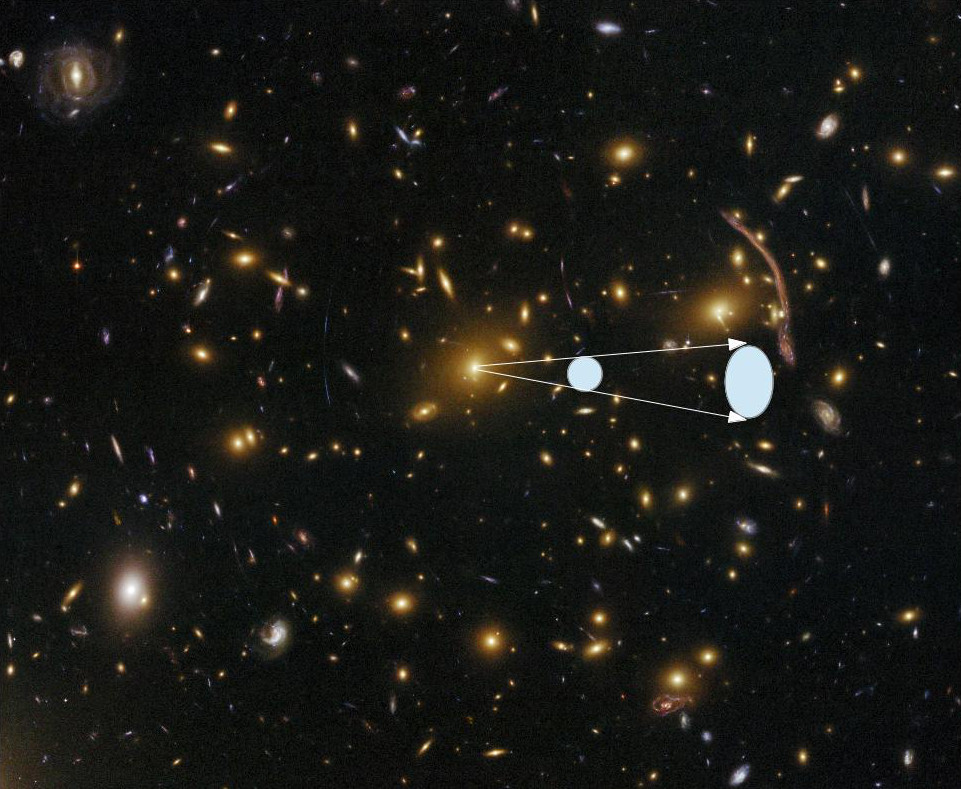
\includegraphics[height=0.8\textheight]{shear-illustration-nowhite.jpg}
        \end{center}
    }

	\definecolor{mblack}{RGB}{50,50,50}
    \setbeamertemplate{background canvas}[vertical shading][bottom=mgray,top=mblack]

}


	
\frame
{
    \frametitle{Shear Illustration}

    \begin{columns}
        \begin{column}{0.5\textwidth}    
            \begin{itemize}

                \item The differential deflections across the surface
                    of the background image produces a ``shear'' in a
                    bundle of light rays.

                \item The shape of extended background sources is changed.

                \item For strong lensing a round source becomes a ``banana''

                \item For {\color{gold} weak lensing} a round source becomes slightly elliptical

            \end{itemize}
        \end{column}
        \begin{column}{0.5\textwidth}
            \begin{center}
                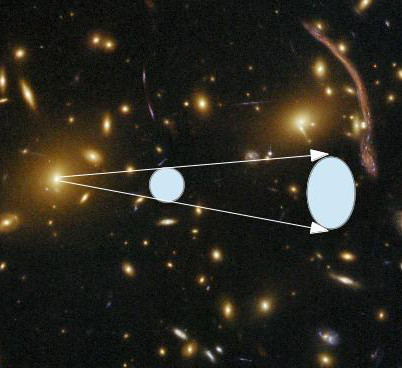
\includegraphics[width=\textwidth]{shear-illustration-crop2.jpg}
                \newline
                {\small Tangential Shear}
            \end{center}
        \end{column}
    \end{columns}
}

\frame
{
    \frametitle{Weak Lensing}

    \begin{columns}

        \begin{column}{0.5\textwidth}
            \begin{center}
                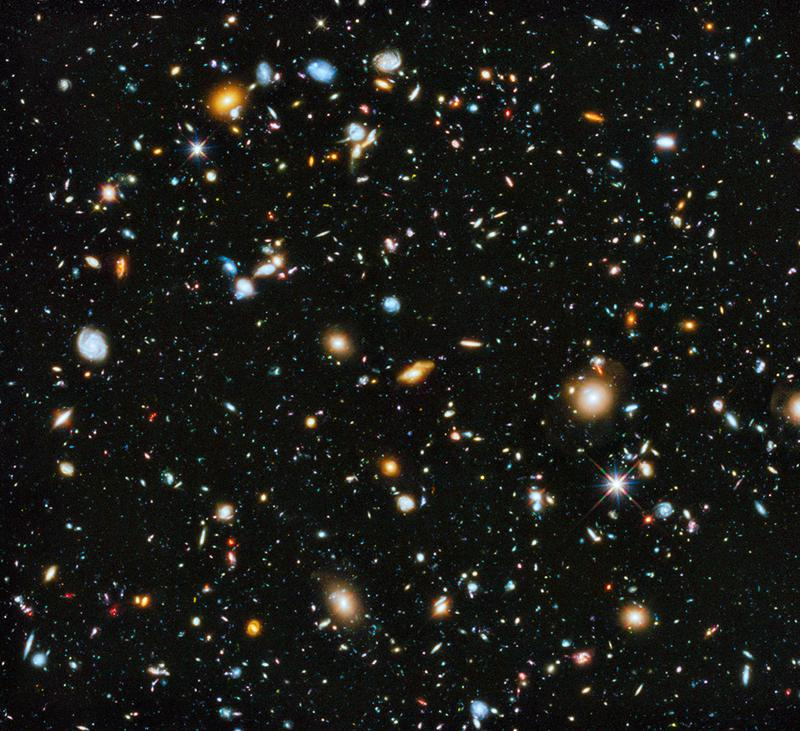
\includegraphics[width=\textwidth]{hubble-ultra-deep-scaled.jpg}
                \newline
                {\tiny  NASA/ESA, Teplitz et al.}
            \end{center}
        \end{column}

        \begin{column}{0.5\textwidth}    
            \begin{itemize}

                \item Strong lensing requires special, fortuitous alignments.
                    % Not that useful as a general tool

                \item But everything is lensed slightly, and the {\color{gold} tangential shear}
                    pattern is imprinted all over the sky.

                \item Taking a statistical approach, we can study the mass
                    distribution around any set of objects.

                \item Can also look for the general pattern on the sky, rather
                    than around specific lenses

            \end{itemize}
        \end{column}

    \end{columns}
}


{
	\definecolor{mblack}{RGB}{0,0,0}
    \setbeamertemplate{background canvas}[vertical shading][bottom=black,top=black]
	
    \frame
    {
        \frametitle{Weak Lensing: Tangential Shear}
            
            \begin{minipage}{\linewidth}
                \begin{center}
                    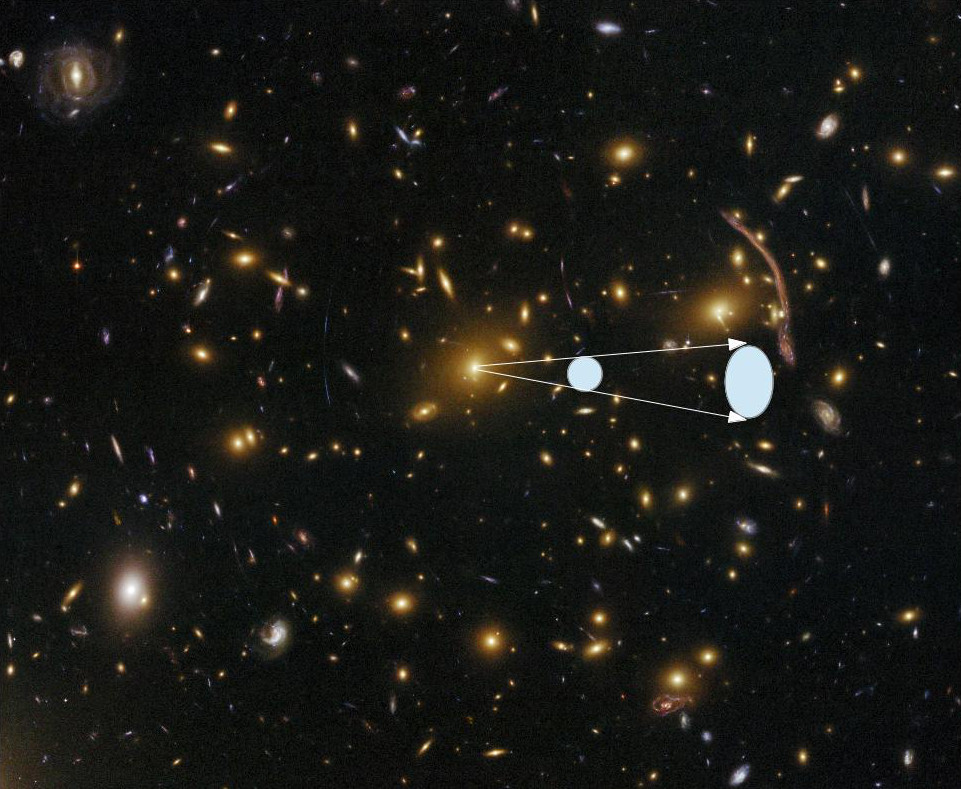
\includegraphics[height=0.6\textheight]{shear-illustration-nowhite.jpg}
                \end{center}
            \end{minipage}

            \begin{minipage}{\linewidth}
                \begin{center}
                    {\color{gold}
                        {\huge
                            $\overline{e}_{T}(R) \propto \overline{\Sigma}(<R) - \overline{\Sigma}(R)$
                        }
                    }
                \end{center}
            \end{minipage}

    }


	\definecolor{mblack}{RGB}{50,50,50}
    \setbeamertemplate{background canvas}[vertical shading][bottom=mgray,top=mblack]

}

\frame
{
    \frametitle{Using Lensing to Measure Dark Energy}

    %\fontsize{9}{0.8\baselineskip}
    \begin{columns}
        \begin{column}{0.5\textwidth}    
            \begin{itemize}

                \item Lensing is geometrical, depends on the distances to all
                    components of the lens system

                \item Look at the dependence of the shear effect as a function
                    of the source redshift
                    
                \item The strength of the signal depends on the amount and
                    properties of Dark Energy

            \end{itemize}
        \end{column}
        \begin{column}{0.5\textwidth}
            \begin{center}
                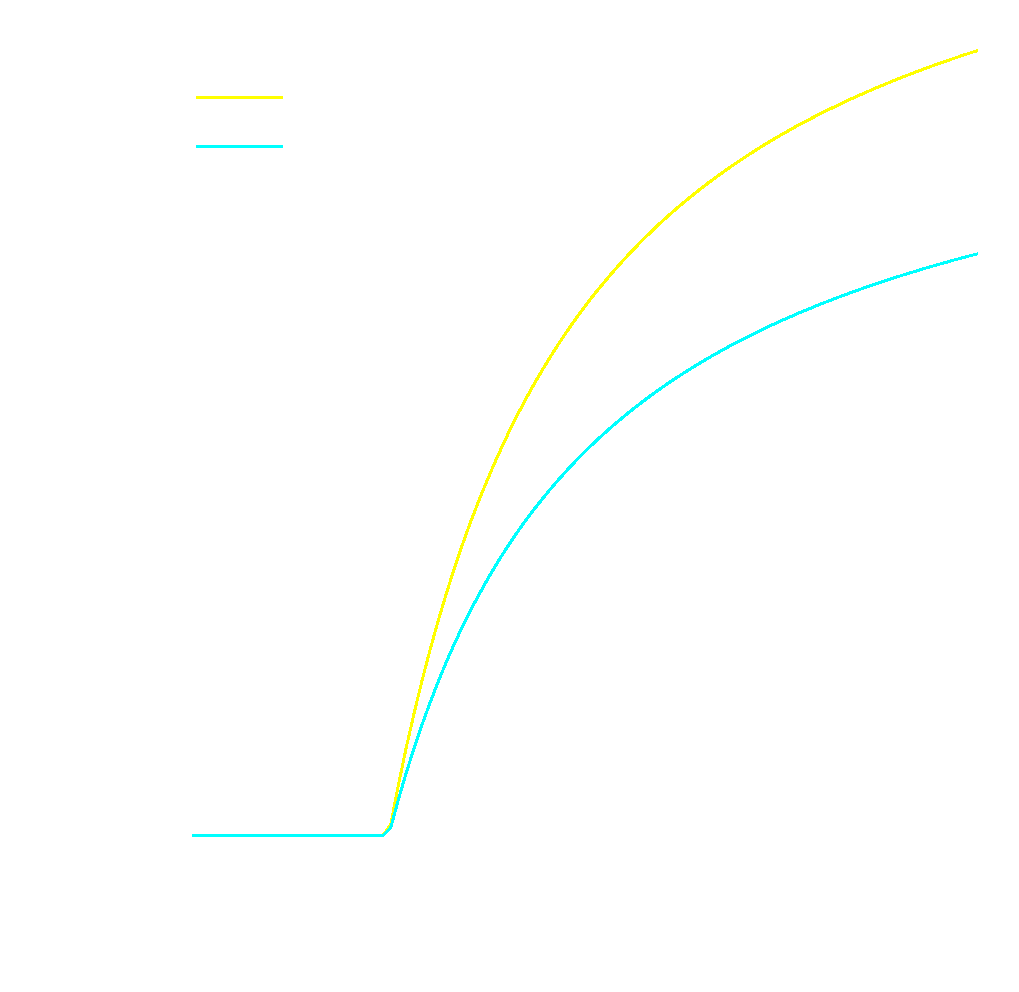
\includegraphics[width=\textwidth]{scinv-example-invert.pdf}
            \end{center}
        \end{column}
    \end{columns}
}

\frame
{
    \frametitle{What do we actually measure?}

    \setbeamerfont*{itemize/enumerate body}{size=\scriptsize}
    \setbeamerfont*{itemize/enumerate subbody}{parent=itemize/enumerate body}
    \setbeamerfont*{itemize/enumerate subsubbody}{parent=itemize/enumerate body}

    %\fontsize{9}{0.8\baselineskip}
    \begin{columns}
        \begin{column}{0.5\textwidth}    
            \begin{itemize}

                \item Its difficult to measure densities directly, such
                    as \gomegam, \glambda, and the variance \gsigma.

                \item Instead we measure the spatial correlations in
                    the lensing signal, which are related to the correlations
                    in the underlying mass density field.


                \item We also look at the cross-correlation between
                    galaxies and the lensing signal, and correlations
                    of the galaxy positions

                \item These correlations can be predicted from the above densities and other
                    cosmological parameters
                    
                \item It is these signals that we examing as a function
                    of distance from us to learn about Dark Energy.

            \end{itemize}
        \end{column}
        \begin{column}{0.5\textwidth}
            \begin{center}
                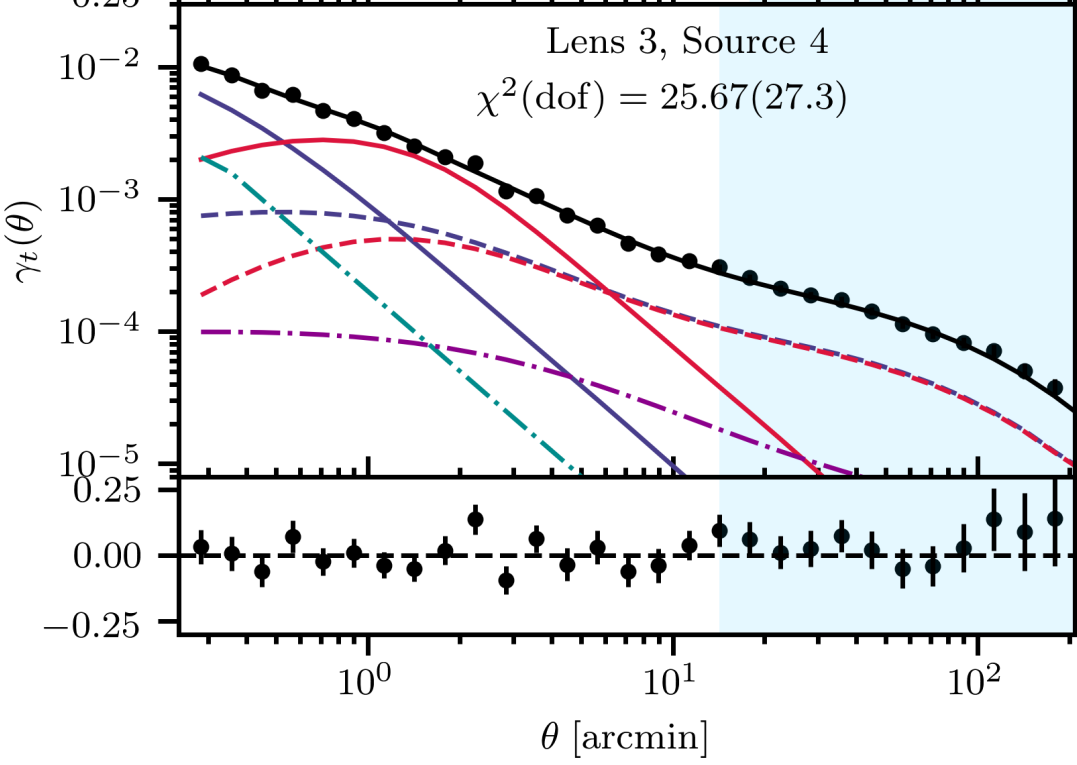
\includegraphics[width=\textwidth]{ggl-example.png}
                Cross-correlation Zacharegkas et al. 2021 (in prep)
            \end{center}
        \end{column}
    \end{columns}
}


\frame
{
    \frametitle{How can we measure shear?}

    \begin{itemize}

        \item Shear induces ellipticity

        \item Ellipticity is also altered by the atmosphere, the optics
            of the telescope, and the pixelization.
        
        \item These effects we call the Point Spread Function (PSF),
            must be modeled by studying stars.

        \item Surprisingly, the noise is the biggest problem:  All
            naive ellipticity measures are biased in the presence of
            noise.

    \end{itemize}
    \begin{center}
        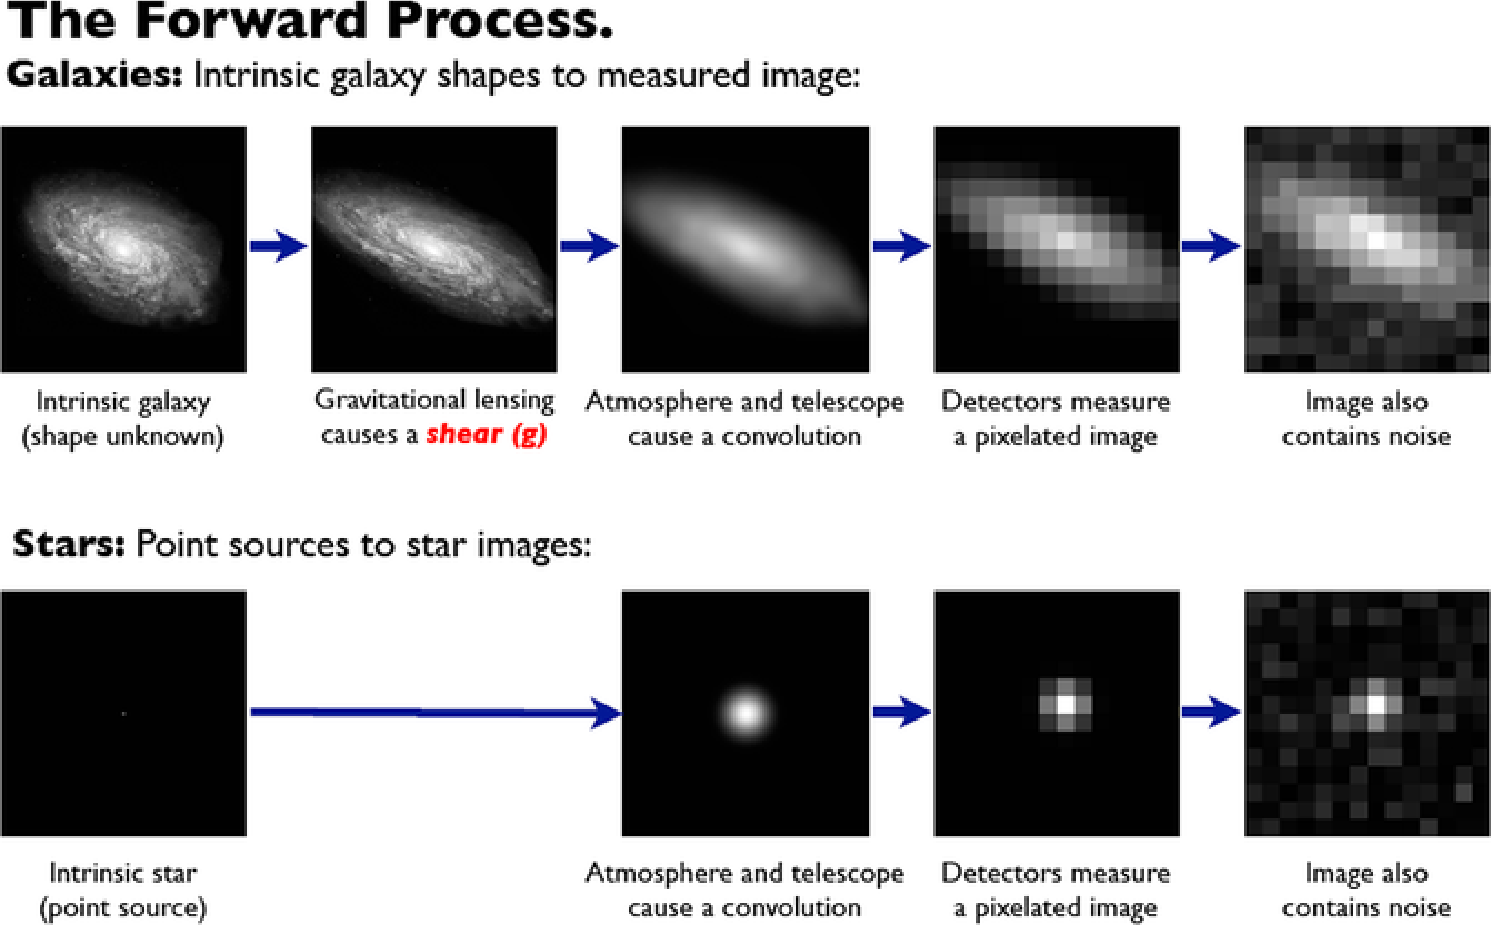
\includegraphics[width=0.7\textwidth]{great08-forward-process.png}
        \newline
        {\tiny GREAT3 Team}
    \end{center}
}


\frame
{
    \frametitle{Calibrating the Lensing Signal}

    % \setbeamerfont*{itemize/enumerate body}{size=\scriptsize}
    % \setbeamerfont*{itemize/enumerate subbody}{parent=itemize/enumerate body}
    % \setbeamerfont*{itemize/enumerate subsubbody}{parent=itemize/enumerate body}

    \begin{itemize}

        \item Basic ellipticity measurements are always biased in the
            presense of noise, and there are significant selection
            effects

        \item In the last few years, colleagues and I have developed a
            technique that is unbiased in principle called
            metacalibration (Huff \& Mandelbaum 2017, Sheldon \& Huff
            2017)

        \item For the work I will show, there is some remaining bias (a few
            percent) that we calibrate with simulations.  Most this bias has
            been addressed with recent improvements, which will be implemented
            for year 6 (Sheldon et al. 2019)

        \item Another promising technique is also in development for
            year 6 (BFD, Bernstein et al. 2014, 2016)

    \end{itemize}

}


\frame
{
    \frametitle{How do we get the redshifts?}

    % \setbeamerfont*{itemize/enumerate body}{size=\scriptsize}
    % \setbeamerfont*{itemize/enumerate subbody}{parent=itemize/enumerate body}
    % \setbeamerfont*{itemize/enumerate subsubbody}{parent=itemize/enumerate body}

    \begin{columns}
        \begin{column}{0.5\textwidth}    
            \begin{itemize}

                \item The prediction of the theory is distance vs redshift, but
                    its too expensive and time consuming to get a spectrum
                    for all galaxies

                \item Galaxies look redder at higher redshift, so we can use
                    the colors to statistically determine the distribution
                    of redshifts

            \end{itemize}
        \end{column}
        \begin{column}{0.5\textwidth}
            \begin{center}
                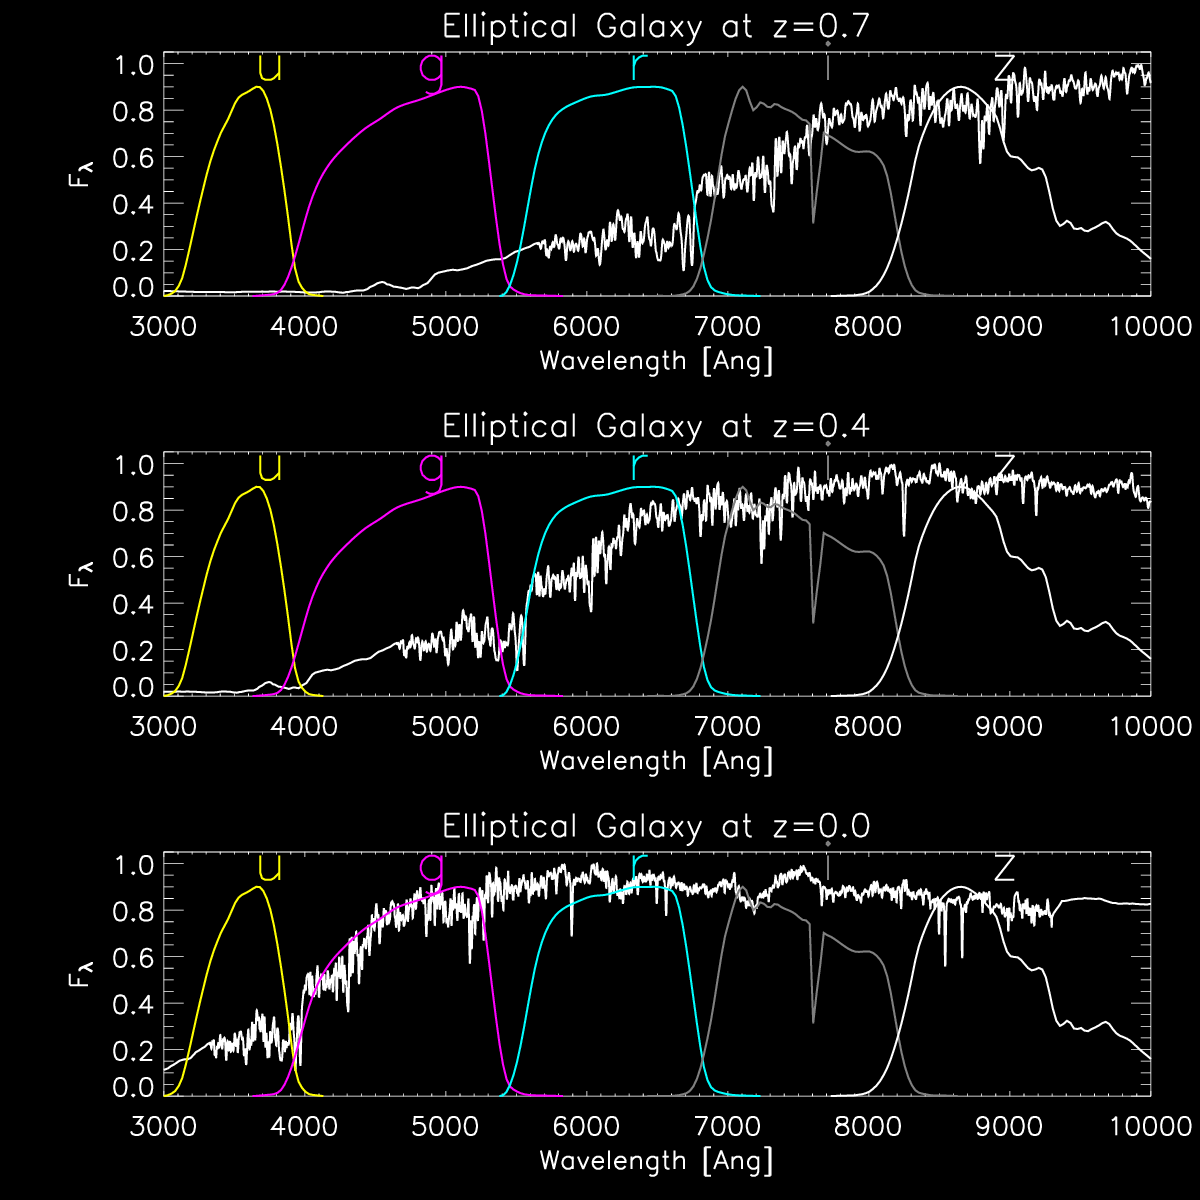
\includegraphics[width=\textwidth]{lrg_spectrum_inv.png}
                {\tiny Padmanabhan (2007)}
            \end{center}
        \end{column}
    \end{columns}


}
\frame
{
    \frametitle{How do we get the redshifts?}

    % \setbeamerfont*{itemize/enumerate body}{size=\scriptsize}
    % \setbeamerfont*{itemize/enumerate subbody}{parent=itemize/enumerate body}
    % \setbeamerfont*{itemize/enumerate subsubbody}{parent=itemize/enumerate body}

    \begin{columns}
        \begin{column}{0.5\textwidth}    
            \begin{itemize}

                \item Clever method to get $P(z | \mathrm{colors})$: Get very
                    deep imaging of objects with known redshifts, then inject
                    images of these galaxies into real data to get
                    $P(\mathrm{color} | z)$ and use Bayes rule

                \item Myles et al. 2021, Gatti et al.
                    2021, Sanchez et al. 2021, DES Collaboration

            \end{itemize}
        \end{column}
        \begin{column}{0.5\textwidth}
            \begin{center}
                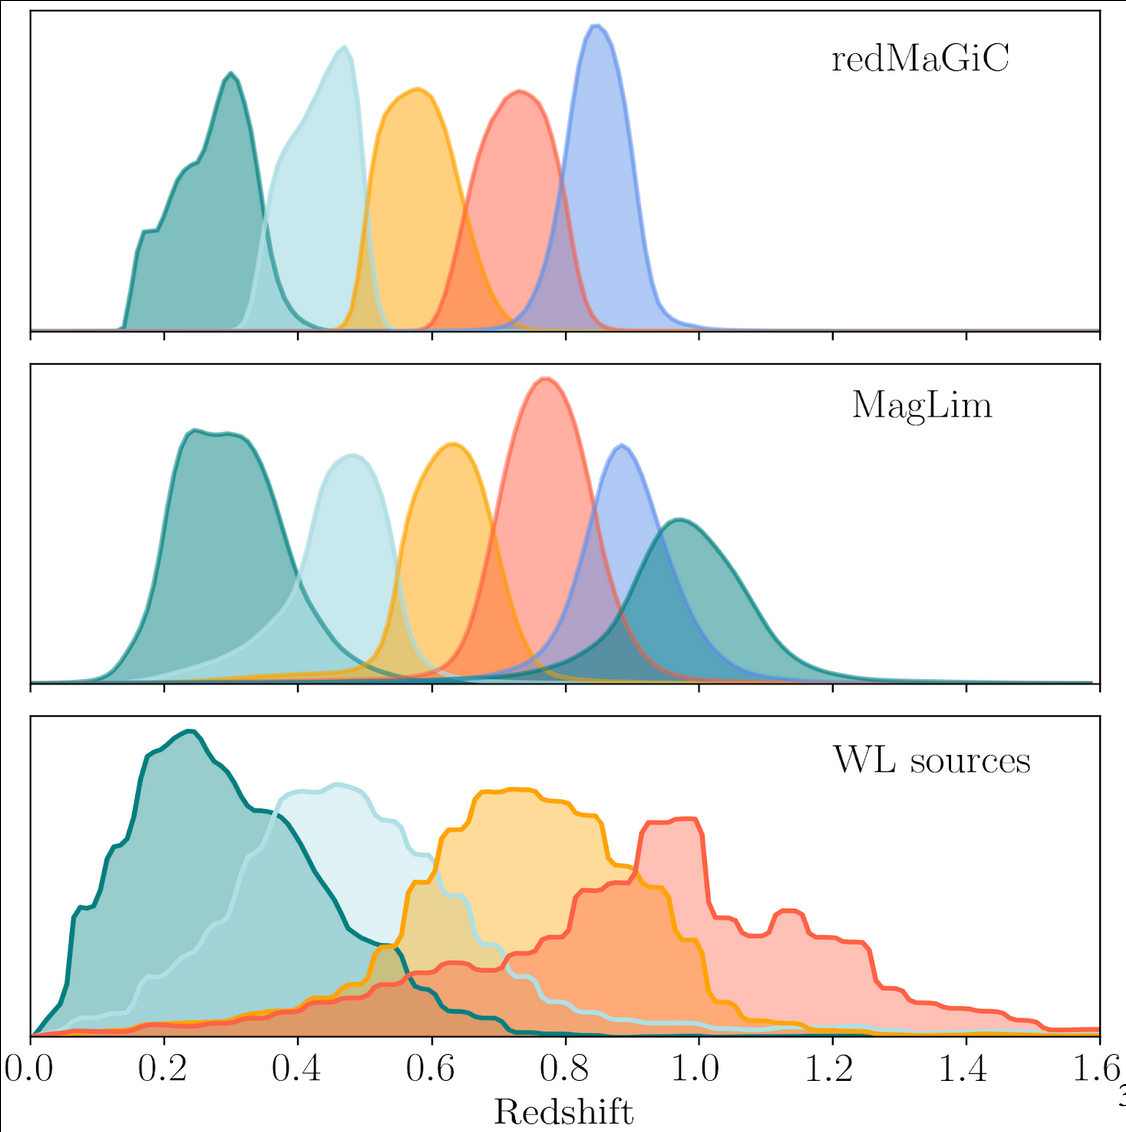
\includegraphics[width=\textwidth]{nz.png}
            \end{center}
        \end{column}
    \end{columns}


}



\frame
{
    \frametitle{Final Calibration from Simulations}

    % \setbeamerfont*{itemize/enumerate body}{size=\scriptsize}
    % \setbeamerfont*{itemize/enumerate subbody}{parent=itemize/enumerate body}
    % \setbeamerfont*{itemize/enumerate subsubbody}{parent=itemize/enumerate body}
    %
    \begin{columns}
        \begin{column}{0.5\textwidth}    
            \begin{itemize}

                \item We have a small, few percent calibration that is determined
                    from semi-realistic simulatons

                \item Put in gravitational shear signals and measure the bias.

                \item Includes effects in the redshift distribution due to
                    blending of background objects with foreground objects

            \end{itemize}
        \end{column}
        \begin{column}{0.5\textwidth}
            \begin{center}
                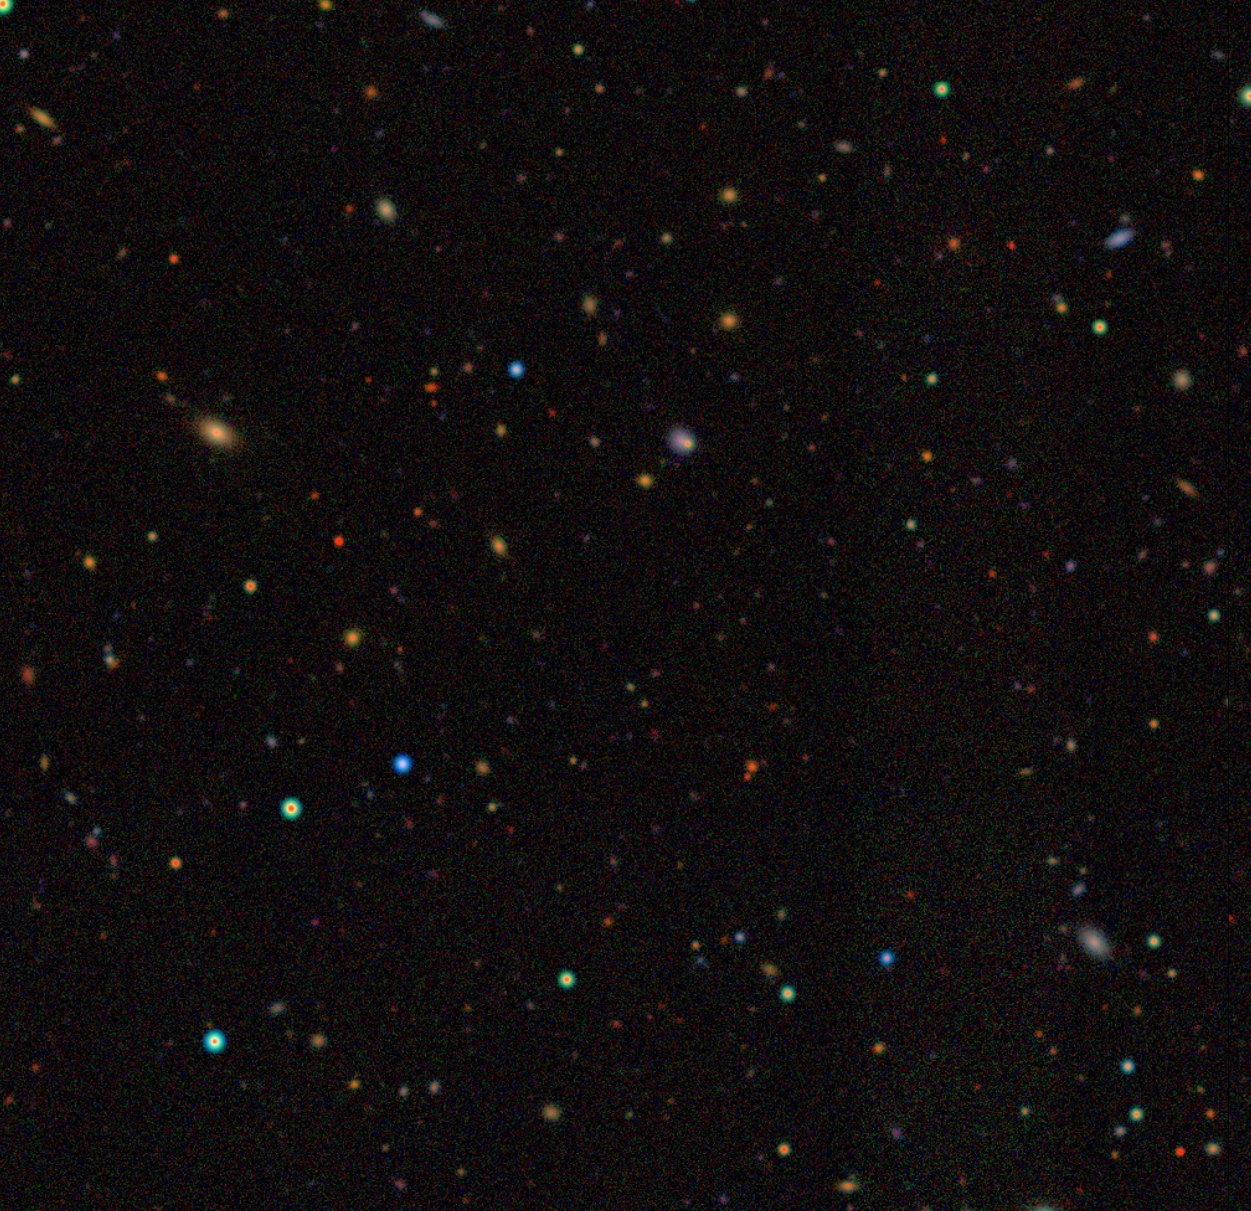
\includegraphics[width=\textwidth]{sim.png}
                {\tiny MacCrann et al. 2021}
            \end{center}
        \end{column}
    \end{columns}


}

{
	\definecolor{mblack}{RGB}{0,0,0}
    \setbeamertemplate{background canvas}[vertical shading][bottom=black,top=black]
	
    \frame
    {
        \frametitle{Simulations}
        \begin{center}
            \includegraphics[width=1.05\textwidth]{simnodivide.png}
        \end{center}
    }

	\definecolor{mblack}{RGB}{50,50,50}
    \setbeamertemplate{background canvas}[vertical shading][bottom=mgray,top=mblack]

}

{
	\definecolor{mblack}{RGB}{0,0,0}
    \setbeamertemplate{background canvas}[vertical shading][bottom=black,top=black]
	
    \frame
    {
        \frametitle{Simulations}
        \begin{center}
            \includegraphics[width=1.05\textwidth]{simdivide.png}
        \end{center}
    }

	\definecolor{mblack}{RGB}{50,50,50}
    \setbeamertemplate{background canvas}[vertical shading][bottom=mgray,top=mblack]

}



\frame
{
    \frametitle{Weak Lensing: The Program}

    \setbeamerfont*{itemize/enumerate body}{size=\scriptsize}
    \setbeamerfont*{itemize/enumerate subbody}{parent=itemize/enumerate body}
    \setbeamerfont*{itemize/enumerate subsubbody}{parent=itemize/enumerate body}

    \begin{columns}
        \begin{column}{0.5\textwidth}    
            \begin{enumerate}

                \item Identify $\sim$foreground galaxies to be lenses

                \item Identify $\sim$background sources and measure their
                    ellipticities % {\color{gold}(that's the hard part!)}

                \item Average the ellipticities of background galaxies

                \item Average over lots of lenses to get the correlation
                    function

                \item Apply calibrations and determine the distribution
                    of redshifts

                \item Interpret in terms of cosmology

            \end{enumerate}
        \end{column}
        \begin{column}{0.5\textwidth}
            \begin{center}
                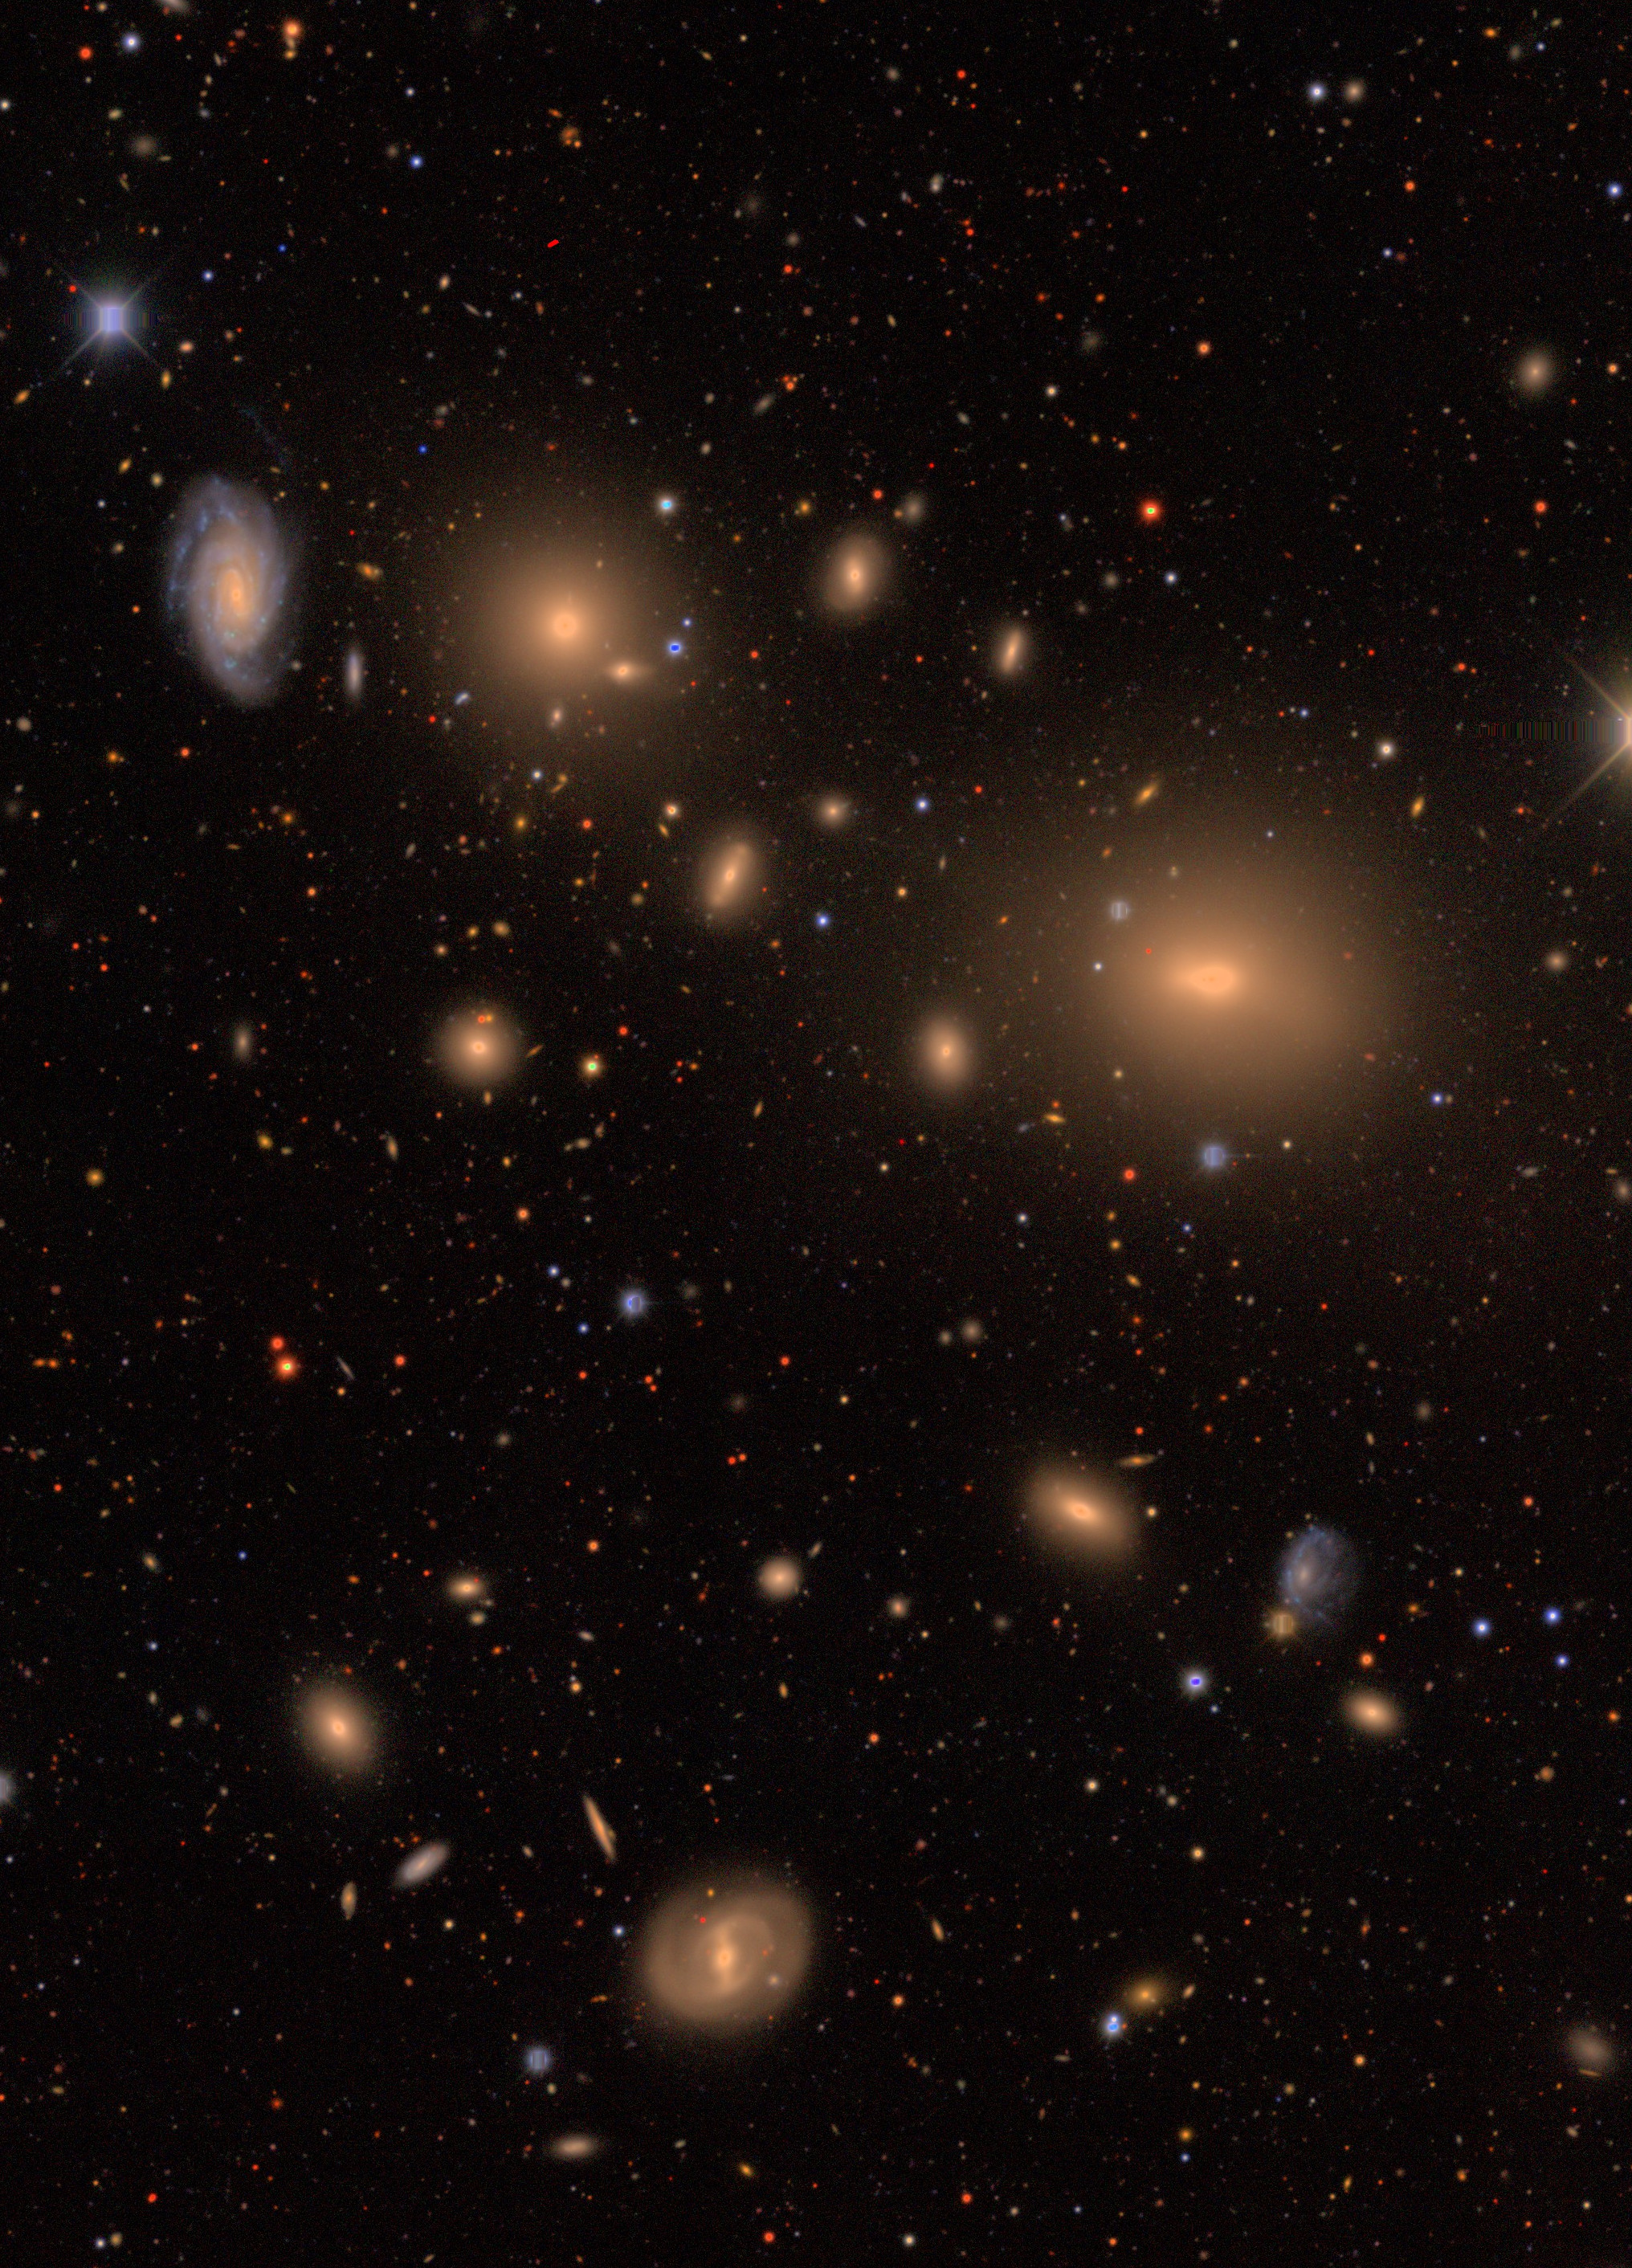
\includegraphics[width=\textwidth]{DES0012-5705-gri-group.jpg}
                \newline
                {\tiny Erin Sheldon, DES}
            \end{center}
        \end{column}
    \end{columns}
}


\frame
{
    \frametitle{Weak lensing ``cosmic shear''}

    \setbeamerfont*{itemize/enumerate body}{size=\scriptsize}
    \setbeamerfont*{itemize/enumerate subbody}{parent=itemize/enumerate body}
    \setbeamerfont*{itemize/enumerate subsubbody}{parent=itemize/enumerate body}

    \begin{center}
        \includegraphics[width=\textwidth]{cosmicshear.png}
        {\tiny Prat et al. 2021}
    \end{center}

    \begin{itemize}

        \item Spatial correlation function of the shapes, corresponds to
            spatial correlation of the mass

        \item On large scales can be predicted in terms of cosmological
            parameters

    \end{itemize}

}

\frame
{
    \frametitle{Cosmology from cosmic shear alone}

    \setbeamerfont*{itemize/enumerate body}{size=\scriptsize}
    \setbeamerfont*{itemize/enumerate subbody}{parent=itemize/enumerate body}
    \setbeamerfont*{itemize/enumerate subsubbody}{parent=itemize/enumerate body}

    \begin{columns}
        \begin{column}{0.5\textwidth}    
            \begin{itemize}

                \item Assuming the dark energy is \glambda, meaning
                    exactly \gw{\color{gold}$~=1$}

                \item Explore 32-dimensional parameter space

                \item Cosmological parameters, but also additional parameters
                    to describe astrophysics (e.g. bias parameters) and
                    systematics with bayesian priors

                \item These are the two cosmological parameters best constrained by our data

                \item Recall {\color{gold} $S_8 = \sigma_8 \left( \Omega_m / 0.3 \right)^{0.5}$}

            \end{itemize}
        \end{column}
        \begin{column}{0.5\textwidth}
            \begin{center}
                \includegraphics[width=\textwidth]{lcdm-xi-ggl-inv.png}
                {\tiny Secco et al. 2021, Abbot et al. 2021, Dark Energy Survey}
            \end{center}
        \end{column}
    \end{columns}

}


\frame
{
    \frametitle{Weak lensing cross-correlation}

    \setbeamerfont*{itemize/enumerate body}{size=\scriptsize}
    \setbeamerfont*{itemize/enumerate subbody}{parent=itemize/enumerate body}
    \setbeamerfont*{itemize/enumerate subsubbody}{parent=itemize/enumerate body}

    \begin{center}
        \includegraphics[width=\textwidth]{ggl.png}
    \end{center}

    \begin{itemize}

        \item Spatial cross-correlation between lens galaxies and
            the shear field (background galaxy ellipticities)

        \item On large scales can also be predicted in terms of cosmological
            parameters

    \end{itemize}

}

\frame
{
    \frametitle{Spatial correlatoin of galaxy positions}

    \setbeamerfont*{itemize/enumerate body}{size=\scriptsize}
    \setbeamerfont*{itemize/enumerate subbody}{parent=itemize/enumerate body}
    \setbeamerfont*{itemize/enumerate subsubbody}{parent=itemize/enumerate body}

    \begin{itemize}

        \item Spatial correlation of galaxy positions 

        \item On large scales, proportional to the correlatoin of the
            mass, but with proportionality factors that must be inferred

    \end{itemize}
    \begin{center}
        \includegraphics[width=\textwidth]{wtheta.png}
        {\tiny Rodriguez-Monroy et al. 2021}
    \end{center}

}

\frame
{
    \frametitle{Combining all three: 3x2pt}

    \begin{center}
        \includegraphics[width=\textwidth]{all.png}
    \end{center}

}


\frame
{
    \frametitle{Cosmology combining all three: 3x2pt}

    % \setbeamerfont*{itemize/enumerate body}{size=\scriptsize}
    % \setbeamerfont*{itemize/enumerate subbody}{parent=itemize/enumerate body}
    % \setbeamerfont*{itemize/enumerate subsubbody}{parent=itemize/enumerate body}

    \begin{columns}
        \begin{column}{0.5\textwidth}    
            \begin{itemize}

                \item The blue shows the results for the lensing cross-correlation
                    and the clustering of galaxies

                \item These results are consistent, so we can combine them 

            \end{itemize}
        \end{column}
        \begin{column}{0.5\textwidth}
            \begin{center}
                \includegraphics[width=\textwidth]{lcdm-xi-ggl-inv.png}
                {\tiny Secco et al. 2021, Abbot et al. 2021, DES Collaboration}
            \end{center}
        \end{column}
    \end{columns}

}

\frame
{
    \frametitle{Cosmology combining all three}

    % \setbeamerfont*{itemize/enumerate body}{size=\scriptsize}
    % \setbeamerfont*{itemize/enumerate subbody}{parent=itemize/enumerate body}
    % \setbeamerfont*{itemize/enumerate subsubbody}{parent=itemize/enumerate body}

    \begin{columns}
        \begin{column}{0.5\textwidth}    
            \begin{itemize}

                \item Now showing is the combined constraints

            \end{itemize}
        \end{column}
        \begin{column}{0.5\textwidth}
            \begin{center}
                \includegraphics[width=\textwidth]{lcdm-xi-ggl-combined-inv.png}
                {\tiny Secco et al. 2021, Abbot et al. 2021, DES Collaboration}
            \end{center}
        \end{column}
    \end{columns}

}

\frame
{
    \frametitle{Comparing to the early universe: CMB}

    % \setbeamerfont*{itemize/enumerate body}{size=\scriptsize}
    % \setbeamerfont*{itemize/enumerate subbody}{parent=itemize/enumerate body}
    % \setbeamerfont*{itemize/enumerate subsubbody}{parent=itemize/enumerate body}

    \begin{columns}
        \begin{column}{0.5\textwidth}    
            \begin{itemize}

                \item Recall the CMB is the relic radiation from the early
                    universe

                \item Good agreement with results from the Planck sattelite (2018)

                \item combined results shown

            \end{itemize}
        \end{column}
        \begin{column}{0.5\textwidth}
            \begin{center}
                \includegraphics[width=\textwidth]{lcdm-compare-planck-inv.png}
                {\tiny Secco et al. 2021, Abbot et al. 2021, DES Collaboration}
            \end{center}
        \end{column}
    \end{columns}

}

\frame
{
    \frametitle{External Consistency}

    % \setbeamerfont*{itemize/enumerate body}{size=\scriptsize}
    % \setbeamerfont*{itemize/enumerate subbody}{parent=itemize/enumerate body}
    % \setbeamerfont*{itemize/enumerate subsubbody}{parent=itemize/enumerate body}

    \begin{columns}
        \begin{column}{0.5\textwidth}    
            \begin{itemize}

                \item We can construct three independent data sets

                \item Lensing and galaxy clustering in DES (3x2pt)

                \item The combination of other low redshift non-lensing
                    data (Supernovae, BAO, RSD)

                \item Planck CMB

                \item Good consistency

            \end{itemize}
        \end{column}
        \begin{column}{0.5\textwidth}
            \begin{center}
                \includegraphics[width=\textwidth]{lcdm-compare-ext-lowz-inv.png}
                {\tiny Secco et al. 2021, Abbot et al. 2021, DES Collaboration}
            \end{center}
        \end{column}
    \end{columns}

}

\frame
{
    \frametitle{DES 3x2pt + lowz + CMB}

    % \setbeamerfont*{itemize/enumerate body}{size=\scriptsize}
    % \setbeamerfont*{itemize/enumerate subbody}{parent=itemize/enumerate body}
    % \setbeamerfont*{itemize/enumerate subsubbody}{parent=itemize/enumerate body}

    \begin{columns}
        \begin{column}{0.5\textwidth}    
            \begin{itemize}

                \item We can construct three independent data sets

                \item Lensing and galaxy clustering in DES (3x2pt)

                \item The combination of other low redshift non-lensing
                    data (Supernovae, BAO, RSD)

                \item Planck CMB

                \item Combine all

            \end{itemize}
        \end{column}
        \begin{column}{0.5\textwidth}
            \begin{center}
                \includegraphics[width=\textwidth]{lcdm-compare-ext-lowz-combplanck-inv.png}
                {\tiny Secco et al. 2021, Abbot et al. 2021, DES Collaboration}
            \end{center}
        \end{column}
    \end{columns}

}



\frame
{
    \frametitle{DES Constraints on Dark Energy equation of state parameter $w$}

    % \setbeamerfont*{itemize/enumerate body}{size=\scriptsize}
    % \setbeamerfont*{itemize/enumerate subbody}{parent=itemize/enumerate body}
    % \setbeamerfont*{itemize/enumerate subsubbody}{parent=itemize/enumerate body}

    \begin{columns}
        \begin{column}{0.5\textwidth}    
            \begin{itemize}

                \item Most precise constraints to date on $w$
                    using lensing and clustering 3x2pt

                \item We can also combine with supernova results from DES

                \item {\color{gold} $w = -0.86 \pm 0.11$} (1-sigma)

                \item Consistent with $w = -1$

            \end{itemize}
        \end{column}
        \begin{column}{0.5\textwidth}
            \begin{center}
                % \includegraphics[width=\textwidth]{wcdm-des-with-sn-crop-inv.png}
                \includegraphics[height=0.7\textheight]{wcdm-des-with-sn-inv.png}
                \newline
                {\tiny Secco et al. 2021, Abbot et al. 2021, DES}
            \end{center}
        \end{column}
    \end{columns}

}

\frame
{
    \frametitle{Combining experiments}

    % \setbeamerfont*{itemize/enumerate body}{size=\scriptsize}
    % \setbeamerfont*{itemize/enumerate subbody}{parent=itemize/enumerate body}
    % \setbeamerfont*{itemize/enumerate subsubbody}{parent=itemize/enumerate body}

    \begin{columns}
        \begin{column}{0.5\textwidth}    
            \begin{itemize}

                \item Combine DES with other low z experiments and the CMB

                \item {\color{gold} $w = -1.03 \pm 0.03$} (1-sigma)

                \item Consistent with $w = -1$

            \end{itemize}
        \end{column}
        \begin{column}{0.5\textwidth}
            \begin{center}
                \includegraphics[width=\textwidth]{wcdm-all-inv.png}
                \newline
                {\tiny Secco et al. 2021, Abbot et al. 2021, DES}
            \end{center}
        \end{column}
    \end{columns}

}


\frame
{
    \frametitle{DES: Future Work}

    \setbeamerfont*{itemize/enumerate body}{size=\Large}
    \setbeamerfont*{itemize/enumerate subbody}{parent=itemize/enumerate body}
    \setbeamerfont*{itemize/enumerate subsubbody}{parent=itemize/enumerate body}
 
    \begin{itemize}

        \item TODO Year 6

    \end{itemize}

}


\frame
{
    \frametitle{The Long View: LSST}

    %\setbeamerfont*{itemize/enumerate body}{size=\Large}
    %\setbeamerfont*{itemize/enumerate subbody}{parent=itemize/enumerate body}
    %\setbeamerfont*{itemize/enumerate subsubbody}{parent=itemize/enumerate body}
    \begin{columns}

        \begin{column}{0.5\textwidth}    
            \begin{center}
                \includegraphics[width=0.90\textwidth]{telescope-summit-april21.jpg}
                \newline
                \includegraphics[width=0.90\textwidth]{Heavy_Lifting_at_Vera_C._Rubin_Observatory.jpg}
                \newline
                {\tiny Rubin Obs/NSF/AURA}
            \end{center}
        \end{column}

        \begin{column}{0.5\textwidth}    

            \begin{itemize}

                \item Vera C. Rubin Observatory,  Legacy Survey of Space and Time

                \item New 3.2 Megapixel camera, the world's largest

                \item New 8.4 Meter telescope

                \item Survey half the sky; 1000 visits per field over 10 years, each
                    with depth of DES 

                \item In construction phase; First light 2022-2023

            \end{itemize}
        \end{column}


    \end{columns}
}

{
	\definecolor{mblack}{RGB}{0,0,0}
    \setbeamertemplate{background canvas}[vertical shading][bottom=black,top=black]
	
    \frame
    {
        \frametitle{Telescope Mount Assembly}
        \begin{center}
            \includegraphics[height=0.7\textheight]{TMA-asturfeito-spain.jpg}
            \newline
            {\tiny TMA assembled at Asturfeito in spain}
        \end{center}
    }

	\definecolor{mblack}{RGB}{50,50,50}
    \setbeamertemplate{background canvas}[vertical shading][bottom=mgray,top=mblack]

}

{
	\definecolor{mblack}{RGB}{0,0,0}
    \setbeamertemplate{background canvas}[vertical shading][bottom=black,top=black]
	
    \frame
    {
        \frametitle{Telescope Mount Assembly}
        \begin{center}
            \includegraphics[height=0.8\textheight]{Some_Assembly_Required.jpg}
            \newline
            {\tiny TMA being re-assembled on the Mountain in Chile,
            Rubin Obs/NSF/AURA}
        \end{center}
    }

	\definecolor{mblack}{RGB}{50,50,50}
    \setbeamertemplate{background canvas}[vertical shading][bottom=mgray,top=mblack]

}


{
	\definecolor{mblack}{RGB}{0,0,0}
    \setbeamertemplate{background canvas}[vertical shading][bottom=black,top=black]
	
    \frame
    {
        \frametitle{Camera}
        \begin{center}
            \includegraphics[height=0.7\textheight]{lsstcam-focalplane-hr.jpg}
            \newline
            {\tiny Camera, electronics made at BNL, camera constructed at SLAC}
        \end{center}
    }

	\definecolor{mblack}{RGB}{50,50,50}
    \setbeamertemplate{background canvas}[vertical shading][bottom=mgray,top=mblack]

}



%\includegraphics[width=\paperwidth,height=\paperheight]{ngc_new_v0-1398_20130130-mm1-2-950px.jpg}}
\usebackgroundtemplate{%
\includegraphics[height=\paperheight]{DES-2013-01-medres.jpg}}
\frame
{

    {\Huge Summary TODO}

    \begin{columns}
        \begin{column}{0.65\textwidth}
            \begin{itemize}
                    {\color{white}

                        %\item Weak lensing is our best method to study the
                        %    distribution of Dark Matter in the universe

                        \item Predictions of Cold Dark Matter theory confirmed
                            \begin{itemize} 

                                \item The distribution of mass in galaxies and
                                    clusters follows a ``universal profile''
                                    
                                \item Universal profile is a running power law, no
                                    exponential cutoff like the light

                                \item Dark Matter is distributed smoothly throughout
                                    the universe, not bound in compact clumps like the
                                    disspiative baryonic material
                            \end{itemize}

                        \item With DES, lensing will mature as a probe of Dark Energy

                        \item This work will culminate in LSST

                    }
            \end{itemize}
        \end{column}
        \begin{column}{0.35\textwidth}
        \end{column}
    \end{columns}
}



\end{document}
